\documentclass[twoside, 12pt]{report}
\usepackage[utf8]{inputenc}
\usepackage{graphicx}
\usepackage{wrapfig}
\usepackage{caption}
\graphicspath{ {figures/} }
\captionsetup[figure]{labelfont={bf},labelsep=period, font={footnotesize, bf}}
\usepackage[a4paper,width=140mm,top=25mm,bottom=25mm,bindingoffset=6mm]{geometry}
\usepackage{apacite}
\usepackage{pdfpages}
\usepackage{nameref}
\usepackage{titling}
\usepackage{csquotes}
\usepackage[T1]{fontenc}
\usepackage{titlesec, blindtext, color}
\definecolor{gray75}{gray}{0.75}
\newcommand{\hsp}{\hspace{20pt}}
\titleformat{\chapter}[hang]{\Huge\bfseries}{\thechapter\hsp\textcolor{gray75}{|}\hsp}{0pt}{\Huge\bfseries}
\usepackage{fancyhdr}
\pagestyle{fancy}
\renewcommand{\chaptermark}[1]{%
\markboth{\thechapter.\textit{\ #1}}{}}
\fancyhf{}
\fancyhead[RE]{\leftmark}
\fancyhead[LO]{\textit {Coupling Action and Function in Games}}
\fancyfoot[RE,LO]{\textbf\thepage}
\fancypagestyle{plain}{%
  \fancyhead{} % get rid of headers
  \renewcommand{\headrulewidth}{0pt} % and the line
}
\setlength{\parindent}{4em}
\setlength{\parskip}{1em}
\renewcommand{\baselinestretch}{1.5}

\bibliographystyle{apacite}

\title{Coupling Action and Function in Games}

\begin{document}

\begin{titlepage}

  \begin{flushright}
    
\includegraphics[width=0.4\textwidth]{ITU_logo}
  \end{flushright}

  \begin{center}

          \vspace*{1cm}

          \Huge\textbf{\thetitle:}

          \vspace{0.5cm}
          \Large Towards a Better Understanding of how to Convey \\
            Meaning Intuitively in Game Design

          \vspace{1.5cm}

          \large
          \textbf{Jonas Haugesen} \\
          \vspace{0.4cm}
          June 2018
          \vfill

          Supervisor: Hans-Joachim Backe, Associate Professor\\

          \vspace{0.4cm}

          A thesis submitted in fulfilment of the requirements
          for the degree of Master of Science.

          \vspace{0.8cm}

          GAMES\\
          IT-University of Copenhagen\\
          Denmark\\
          \vspace{2cm}

      \end{center}
\end{titlepage}

\chapter*{Abstract}
NaN

\noindent
\textbf{Keywords:}
Games


\section{Problem}
The research fields of feedback, feedforward and affordances have been explored within the context of interaction design since at least 1988, but within the context of games, research has been limited yet its application is apparent in games today. In the following thesis, I will cover existing theory within the fields of both game design and interaction design and bridge the gap between the two in the context of the terms feedforward and feedback. I will also apply my research to the creation of a prototype, which will require research of its own within the fields of game design and prototyping. For the prototype, I will also apply theory to the creation of puzzles since puzzles lend themselves well for researching usability because of their high complexity as a challenge. For the evaluation of the applied theory in the prototype I will conduct interviews and play-testing and for this, I will apply theory on testing and qualitative as well as quantitative data and how to acquire this data from the interviews and play-tests.

\section{Method}
Initially, a study of existing theory will form the basis of the formulation of the rest of progress. The status quo of multiple fields of research will be examined and an attempt at extracting a framework of how to best design for a tight coupling between action and function will be made. this will then lead directly to the next phase: Prototyping. By extracting the relevant knowledge in the area, a prototype will be created with the intent of applying previously examined theory. The prototype will consist of multiple challenges with two variations: 1) Using the best practice in relation to the previously extracted framework. 2) Using either a direct opposite of the previous framework or the framework with one or more altered elements. Once the prototype has been created, the applied theory within the prototype will be evaluated by conducting play-tests followed by interviews according to the status quo of this area. The results of the evaluation will then be analysed and form the basis for any conclusion.


\chapter{Theoretical Background}

Meta

\section{Discoverability and Understanding}
\citeA{norman} identifies two properties of design: \textit{Discoverability} and \textit{understanding}. Discoverability is the design's probability of an agent comprehending the possible and intended interaction. For the design to have good discoverability it must communicate the proper information and only this. Understanding is the design's ability to make an agent understand why and how it works. For the design to have good understanding, it must learn the agent why the intended interaction works and perhaps more important why the unintended does not. These two properties are achieved by applying six psychological concepts. For discoverability there are five distinct concepts: \textit{affordances, signifiers, constraints, mappings} and \textit{feedback}. For understanding there is the concept of \textit{conceptual models} \cite{norman}. To fully unearth the properties of discoverability and understanding, I will clarify the definition of all of these six concepts. Before that, however, it is important to note that \citeA{norman} defines these concepts with the lens of how to utilise them to achieve good design, so that while the concepts are presented as universal to all design, the evaluation of how to utilise the concepts for achieving good design is subjective.

\paragraph{Affordances} These are the relationships between the design object and the agent interacting with it. Human-centred design (HCD) would therefore have affordances that describe the relationship between humans and a design object. As an example, a push and pull door may have a handle on one side and not the other: The handle affords a grasping of the handle by a human, which in turn is necessary for the human to be able to pull the door open. The side with no handle does not afford grasping. This is described as an anti-affordance, i.e. the prevention of an interaction \cite{norman}. Without the affordance of grasping the affordance of pushing should persuade the agent. If there had been handles on both sides of the door - thereby communicating wrong information on one side - this would likely lead to an amount of confused humans who would pull where one should push, and would be an example of misleading discoverability \cite{norman}.

\paragraph{Signifiers} Any affordance that cannot be could benefit from another type of communication to make the agent aware of it. \citeA{norman} describes this a signifier. A signifier can be any perceivable indicator that instructs the agent of the possible and intended behaviour \cite{norman}. Staying with the previous example of a push and pull door: A typical example of a signifier being used in this context is the 'push' or 'pull' signs placed somewhere obvious on the door. These signs signify the intended interaction with the door. Signifiers can also be something more abstract, like footprints in the snow, signalling the preferred route from point A to B \cite{norman}.

\paragraph{Mappings} In mathematics, mappings are ``[...] the relationship between the elements of two sets of things'' \cite[p. 20]{norman}. In design, mapping is relevant when designing the layout of controls and displays. \citeA{norman} defines a good use of mapping in design as having spatial coherence between the layout of the controls and the elements that they control. In some modern 3D video games that use a dual analogue controller, a mapping is applied by the left analogue stick moving the player's avatar in its tilted direction and the right analogue stick rotating the view in its tilted direction. When designing for mapping one can use the techniques of \textit{grouping} and \textit{proximity} by grouping together related controls and by placing the control near the element that it controls \cite{norman}.

A \textit{natural mapping} \cite{norman} is a concept used for describing a design ``[...] where the relationship between the controls and the object to be controlled [...] is obvious'' \cite[p. 115]{norman}. In the original Pokémon Blue Version game \cite{pokemon}, the player controls a character in the centre of the screen in a top-down perspective. The device it was made for, the Game Boy, has a four-directional button and these four directions are mapped naturally to the character's movement on screen (see figure \ref{pokemon}).

\begin{wrapfigure}{i}{0.35\textwidth}
  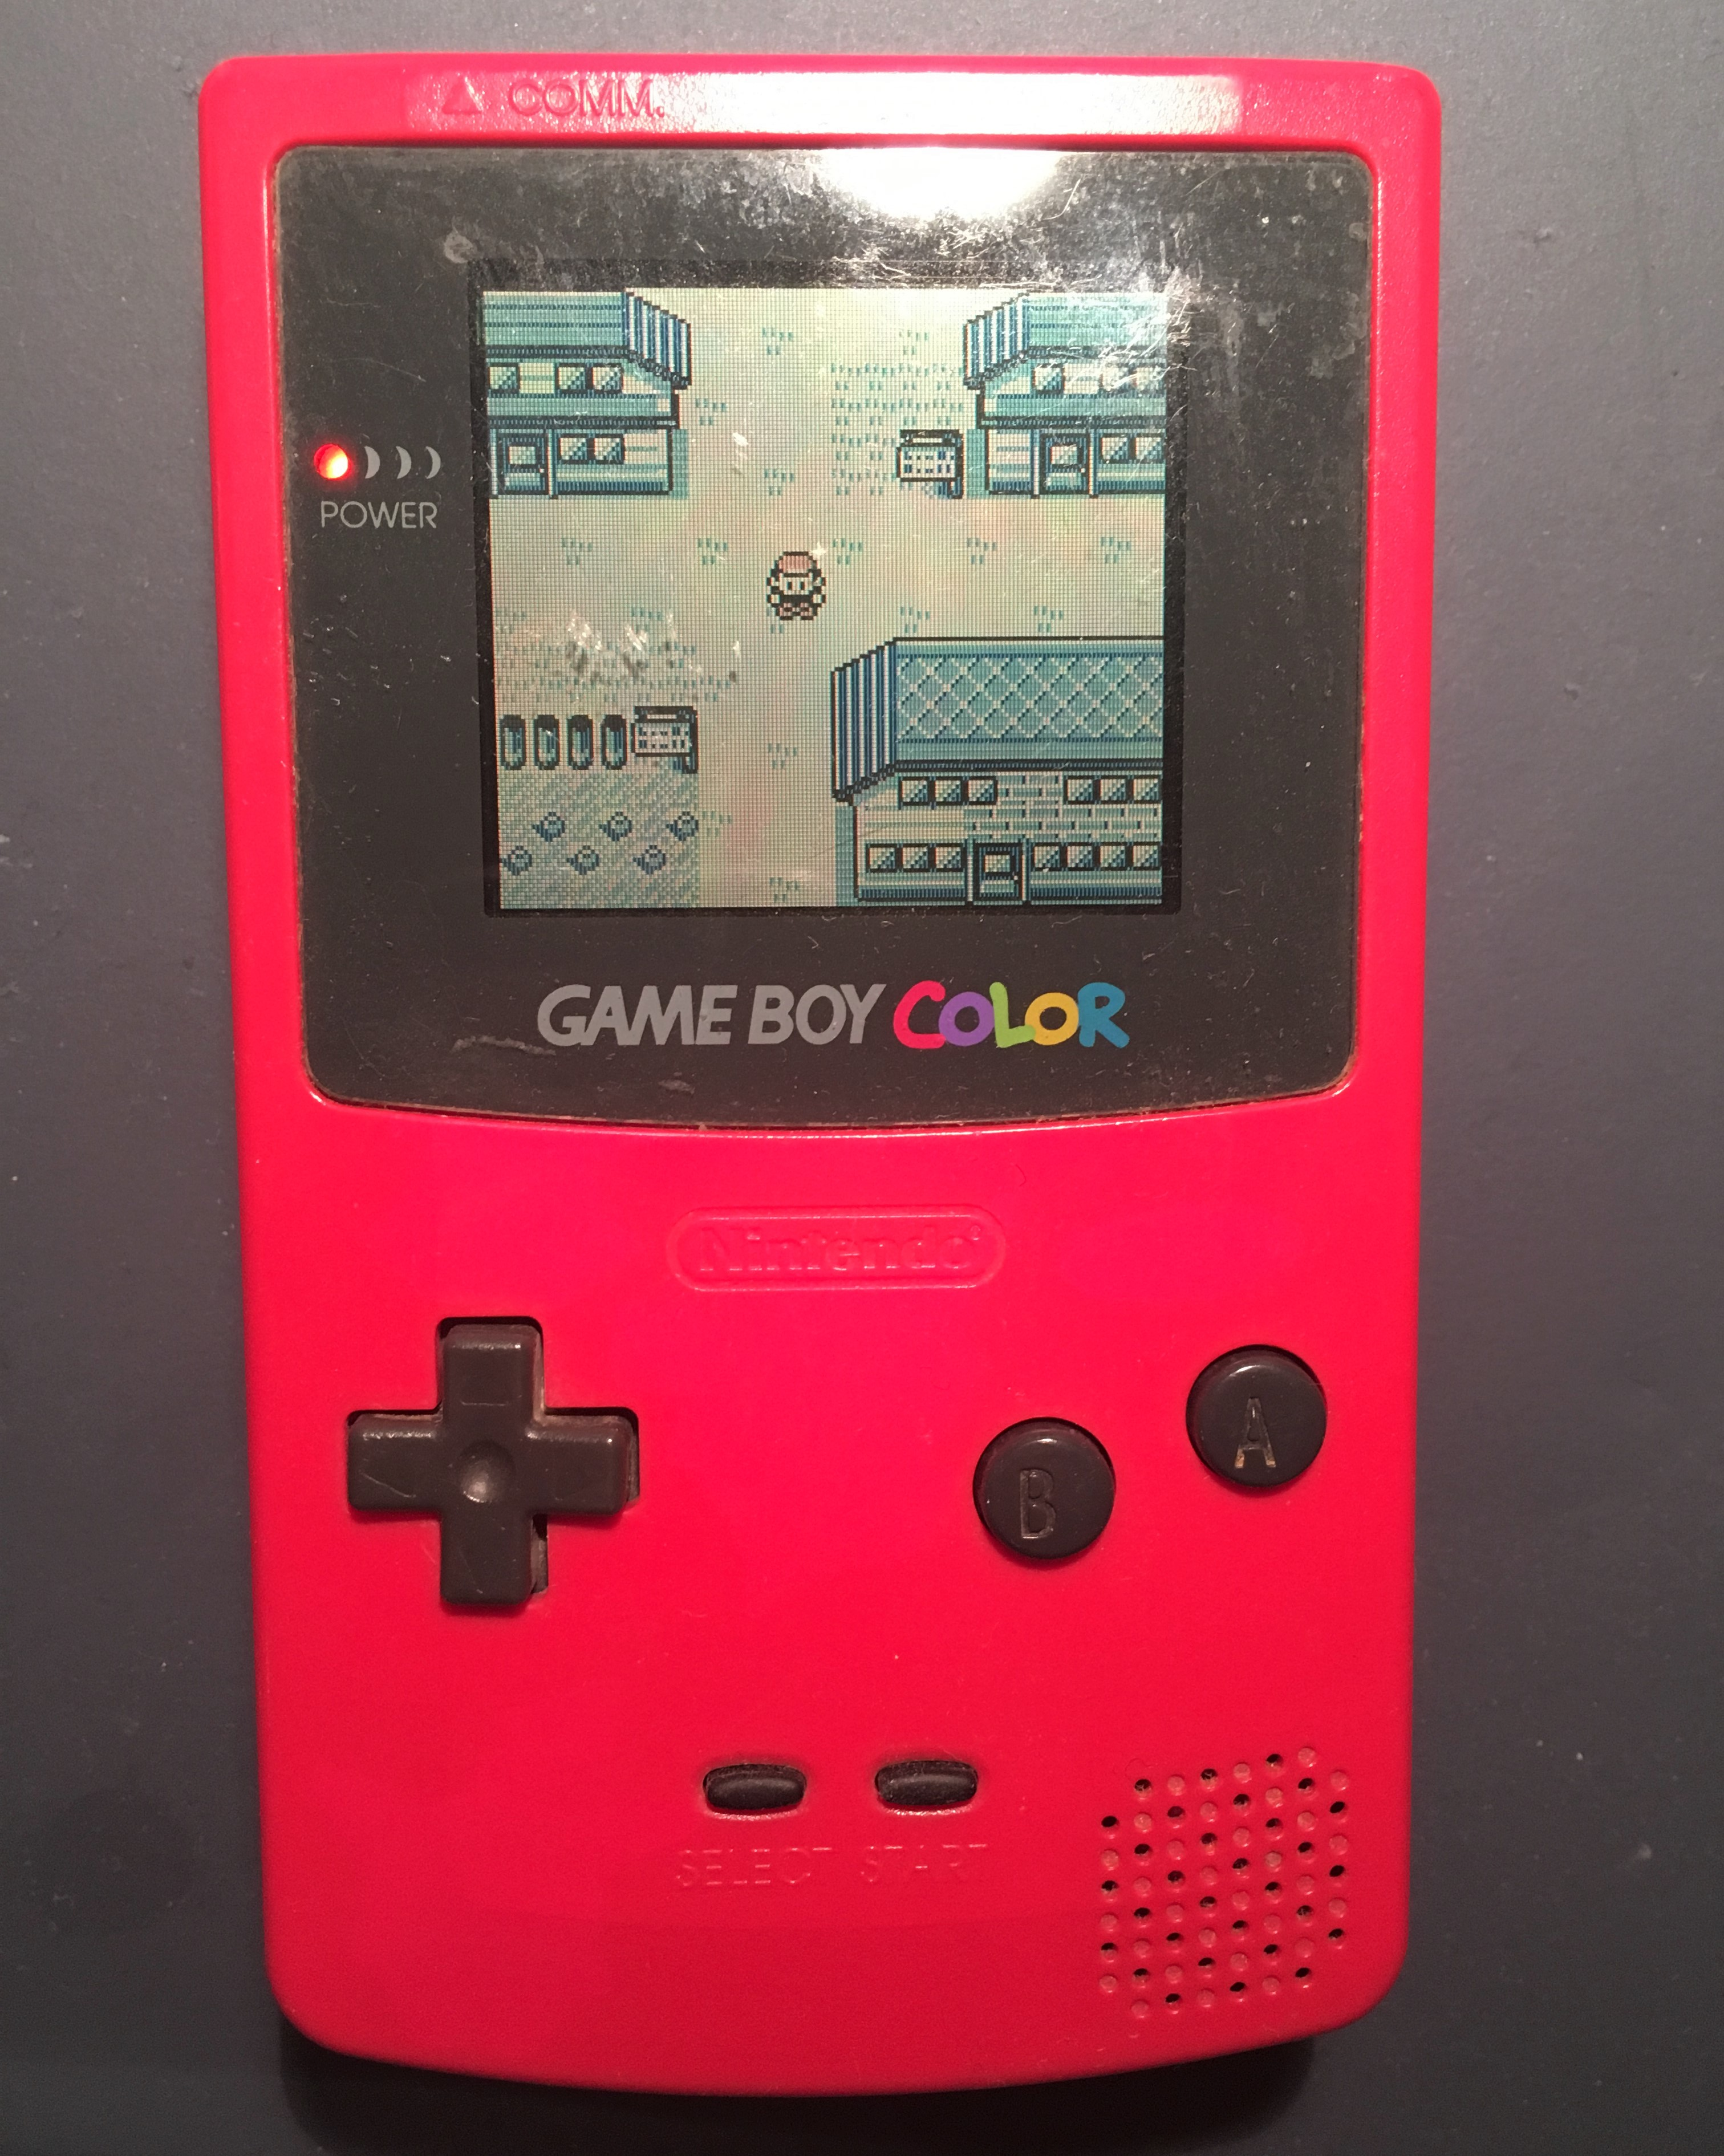
\includegraphics[width=0.35\textwidth]{Pokemon}
  \caption{Pokémon Blue Version playing on a Game Boy}
  \label{pokemon}
\end{wrapfigure}

\paragraph{Constraints} \citeA{norman} defines constraints as being four-part: Physical, cultural, semantic and logical. The physical limits of a design, constrain the possible interactions with it \cite{norman}. Consider a regular scissor: It has two holes for inserting fingers. One is large and the other smaller. The smaller hole constrains the number of fingers that may be inserted into it, thereby signifying the proper interaction method. The regular scissor is also an example of how physical constraints can be useful in preventing incorrect actions.

Cultural constraints are when culture provides a set of written and unwritten rules which affects the way a person may interpret a situation. A person from Greece may greet a friend differently than a person from Denmark. In design, these guidelines also act as constraints \cite{norman}. As an example, the difference in right- and left-hand traffic. This cultural constraint has led to cars in Japan, a left-hand traffic country, being designed with the driver's seat in the left side, which is the opposite in Germany, a right-hand traffic country. A Japanese tourist renting a car in Germany, without knowing this cultural difference, would walk to the left side of the car to start the engine. In Japan, the constraint also affects the way people navigate on foot: Going up or down stairs, people keep to the left, which for a tourist from Germany may lead to some unexpected physical constraining.

Semantic constraints are when, as an example, using a regular claw hammer the situation constrains the interaction. If the user is about to hammer in a nail, the user is inclined to use the flat side of the hammer. If the user accidentally bends the nail and wants to extract it, the user is inclined to use the claw. This is a semantic constraint. \cite{norman}.

Logical constraints are closely connected to the concept of natural mapping \cite{norman}. In the case of the Game Boy and Pokémon as discussed earlier, the device provides five visible buttons, excluding volume and power, two of them are circular and grouped on the right side, another two have the appearance of slim lines and the fifth and final has a cross-shape pointing up, down, left, right. When faced with the problem of how to move the character, the logical constraint that \textit{no other button points in directions}, should guide the player towards the cross-shaped button.

\paragraph{Feedback} Feedback describes the information that is relayed back when an action has occurred. In design, it can be utilised to let the user know that her input has been received and/or let the user know the consequence of the action. \citeA{norman} argues that feedback should be immediate and informative. Imagine hitting a button to turn on the light and having no other immediate feedback than the tactile sensation of the button being pressed in and springing back out. There is a delay between the button press and the light turning on, but you do not know this. You wait for a while for the light to turn on, but get impatient. You press again, confused, and still, nothing happens since you have unbeknownst turned off the light before it was able to light up. This is an example where the feedback is not immediate and there is no way for the user to know if her input has been received. Take the same example, but swap the button with a switch and take away the delay. Now, you push the switch and get the immediate feedback of the switch being in an altered state and the light turning on. The switch is more informative than the button since it can be in two different states, mimicking the light that can be either on or off. Another aspect to keep in mind when designing feedback is that too much feedback can end up confusing the user \cite{norman}. Complex systems can accumulate an abundance of information and relay a great deal of this back to the user, which can result in overburdening and confusing the user. This means that design that deals with much information need to prioritise and plan its feedback so that important trumps less important information and that all feedback is not presented in the same instance \cite{norman}.

\paragraph{Conceptual Models} A toaster is a device that many of us know how to operate. The common toaster is operated by pulling down a lever that lowers a slice of bread and exposing it to radiating heat. Suppose a toaster is delivered to a secluded tribe deep in the Amazon. It would be within reason to argue that the tribe would have no clue to what it was for and more importantly: how it works. A conceptual model is a simple explanation, that resides in our minds, of how something works. The reader of this would, in most cases, have a conceptual model of how a common toaster works and would be able to use that understanding to operate said toaster. The residents of the aforementioned tribe would, however, not have such a conceptual model, and would therefore not be able to operate the toaster, disregarding the probable lack of electricity anywhere near them. A conceptual model is, however, not just a model of how something is used properly, but also a model of what makes the thing work. Staying with the toaster example, the reader will presumably know that the lever that lowers the bread, is coupled with a spring that is locked down when the lever is lowered sufficiently. Let us conceive of a situation where you lower the lever of a toaster and assume that the lever is lowered sufficiently, however, it is not. The lever springs back up since the spring has not been locked down. With your conceptual model of the toaster, you surmise that the lever was not lowered enough for the spring to be locked down, and you attempt the lowering once more, making sure to check for the tactile feedback of the locking mechanism. This is an example of a conceptual model providing the knowledge to evaluate a failed interaction and calibrate the approach to successfully carry out the intended operation. ``Conceptual models are valuable in providing understanding, in predicting how things will behave, and in figuring out what to do when things do not go as planned'' \cite[p. 28]{norman}. The question of how one obtains a conceptual model is then relevant. \citeA{norman} defines the \textit{system image} as the image from which one gain a conceptual model. The system image is perceived through all the available material describing the object: documentation, signifiers, the object's physicality, ``what was told to us in the sales literature, by salespeople and advertisements, by articles we may have read, by the product website and instruction manuals'' \cite[p. 31]{norman}, et cetera. It is then the role of the designer to as closely as possible match her own conceptual model with the user's through the utilisation of the system image \cite{norman}.

\newpage


\section{Purpose and Coupling}
With these concepts defined by \citeA{norman} there is a strong foundation for creating a game design framework, however, these concepts focus solely on communicating how something works: "You can figure out the scissors because their operating parts are visible and the implications clear. The conceptual model is obvious, and there is an effective use of signifiers, affordances, and constraints" \cite[p. 27]{norman} but how does one realise that a scissor is for cutting paper? \citeA{norman} does not describe how a design can communicate its purpose. Furthermore, when \citeA{norman} writes that the fact that a scissor's operating parts are visible make the scissor intuitive, an interesting point is made but is not further explored in \citeA{norman}. In \citeA{normanold}, the reason for what makes the scissors intuitive could be described by the concept of \textit{visibility}, but this concept seems to have been incorporated into the more general concept of signifiers. \citeA{howdonald} and \citeA{frogger} offer a more detailed explanation with their definitions of \textit{feedforward} and \textit{feedback} with their subdivisions \textit{inherent, augmented} and \textit{functional}. I will describe their definitions and particularly the subdivisions of \textit{functional feedforward} and \textit{inherent feedback} since I have identified them as crucial in the development of a game design framework. I will furthermore delve into their definitions of these two concepts in correlation to the concepts of \citeA{norman} because they themselves consider the concepts as building on top of the notions of \citeA{normanold}, and because Norman's concepts have been revised \cite{norman} after the fact. A major revision to regard is the addition of the concept of signifiers and the alteration of the definition for affordances. \citeA{norman} notes about affordances that "alas, the term became used in ways that had nothing to do with the original" \cite[p. 13]{norman}. He argues that the design community understood the term as a property instead of a relationship when it needed a term to describe the addition of instructional elements. Therefore, signifiers were termed and affordances were made more concrete. The more broad understanding of affordances is, therefore, the one that is present in \citeA{howdonald} and \citeA{frogger}. However, the arguments and definitions are still relevant for the bolstering of my design framework, since the insights made, do not overlap directly with the old or new insights of \citeA{norman}, but instead expand the research field.

\subsection{Feedforward} Feedforward is the information an object gives before the interaction concerning what the consequences of an action will be. This is given both by the way the object looks, but also the action that it requires \cite{frogger}. It is distinct from perceivable affordances in the way that feedforward informs about what the results of a user's action will be, i.e. the purpose of an action \cite{vermeulen}. To further describe the concept of feedforward, \citeA{frogger} divide the concept into three subdivisions:
\paragraph{Inherent} Resembles perceivable affordances \cite{norman} in the sense that it communicates the action possibilities of the design, but additionally how this action can be made and what it is for \cite{frogger}. It is, importantly, part of the interaction, thereby making the information inherent to the interaction and consequently it appeals to the perceptual-motor skills of the user.
\paragraph{Augmented} Communication about the action possibilities and the purpose of the action coming from an additional source \cite{frogger}. As an example, a lit button next to an elevator shaft communicates to the awaiting future passengers that the car will make a stop at this floor. The light inside or next to the button would be augmented feedforward since it is remote from the actual elevator car, but gives information about the goal of the future passengers: To enter the elevator. This kind of information thusly relies on the user's cognitive abilities since it is the user that needs to know that the light near or on the button indicates that the elevator will stop at his or her floor. This, \citeA{norman} would describe as a signifier.
\paragraph{Functional} In contrast to signifiers, that communicates how and where, functional feedforward communicates the general purpose of the design, i.e. why to do the action \cite{frogger}. Functional feedforward can utilise the concept of \textit{product semantics} \cite{semantics}, where the user's previous experience is relied upon for her to find meaning in the design. Additionally, as described in the scissor example from earlier, functional feedforward can describe the communication that happens when the operating parts are visible to the user, thereby making the function clear \cite{frogger}.

In \citeA{howdonald}, the application of functional feedforward (at this point only described as feedforward) is further explained as follows: The designer must create meaning for the user, and for this, there are two approaches: 1) The semantic approach and 2) the direct approach \cite{howdonald}. 1) The first approach relies on the user's previous experiences and applies that to inform the user of its own resemblance to that previous experience. It often benefits from the use of iconography and symbols \cite{howdonald}. This approach resembles signifiers, and a product of this approach could presumably be interpreted as both a signifier and functional feedforward. 2) The direct approach instead, relies only on bodily and perceptual skills and the intention being that meaning should be created in the interaction. Since perceptual and bodily skills are relied upon, the approach requires tangible interaction \cite{howdonald}. The approach utilises the concept of natural mapping because of the way the spatial layout of a design can communicate the purpose of an action. Spatial layout, however, is just one utilisation of this approach. \citeA{howdonald} describe an example of this approach where part of a design is used to silence the sound it emits: The operating part is placed on top of where a loudspeaker is emitting the sound from, and the loudspeaker is thereafter silenced. The purpose of this action is communicated naturally since it is common knowledge that placing a physical object on top of something that emits sound, obstructs the sound being emitted. This example can be said to use the most effective level of mapping (best mapping) \cite{norman}, but mapping only communicates the spatial relationship between the controls and the controlled, not the meaning of the action.

For applying feedforward in a design, \citeA{howdonald} argues that the direct approach should be prioritized. It takes behaviour and action as its starting point. Instead of focusing on semantics where cognitive skills are relied on to find meaning in resemblance, the authors instead believes that meaning is created in the interaction and thereby relying on perceptual and bodily skills put less strain on the user \cite{frogger}.

\subsection{Feedback} The definition of feedback in \citeA{frogger} is similar to that of \citeA{norman}. The distinction lies is in the three subdivisions of feedback:
\paragraph{Functional} The feedback the user receives concerning the desired functionality of the user \cite{frogger}. If the user performed an action to turn on a light, a light turning on would be the functional feedback.
\paragraph{Augmented} This is feedback coming from an additional source \cite{frogger}. In the elevator example from earlier, the button lighting up when pressed would be augmented feedback, communicating that the car will stop on this floor. The actual consequence of the car stopping on the desired floor would be functional feedback.
\paragraph{Inherent} Inherent feedback means that the performed action and the feedback it gives is closely coupled. The inherent feedback of an action acts as an innate consequence of that action. Unlike augmented feedback, inherent feedback comes from the action itself. The feedback appeals to the perceptual motor skills of the user and can be received visually, auditorily and haptically.

\subsection{Coupling}
Consider the scissor example from earlier once more: When operating a scissor the feedback the user receives is through all of her perceptual motor skills: The incision point of the blades and the paper is visible, the sound of the paper splitting is heard, the haptic feel of the resistance is felt and the blades follow the motion of your hand and fingers. This close coupling of action and meaning is logically always apparent in mechanical products, and makes them intuitive because action and meaning is unified on the six aspects of time, location, direction, dynamics, modality and expression through inherent information \cite{frogger} \cite{transbehav}:
\begin{itemize}
  \item \textit{Time}: The action and meaning takes place at the same time.
  \item \textit{Location}: The action and meaning takes place at the same place.
  \item \textit{Direction}: The direction of the action and meaning is the same.
  \item \textit{Dynamics}: The speed, acceleration and force of the action is closely coupled to the speed, acceleration and force of the meaning.
  \item \textit{Modality}: The sensory modalities (appearance, sound, taste, feel, etc.) of the action are mirrored in the meaning.
  \item \textit{Expression}: Any expression is apparent in both the action and the meaning.
\end{itemize}

Electronic products, \citeA{frogger} argues, can take advantage of these six aspects of coupling to make the interaction more intuitive, by coupling the action and function through augmented and inherent information. What it lacks, is the direct coupling between action and function through inherent information that a scissor as an example would have. To illustrate how a design can be regarded through these six aspects, I will return to the elevator setting from before, instead now the use has arrived in the elevator car. Here the action would be the pushing of a button with the intend of directing the elevator car to the indicated floor, and the function, being transported to that floor:
\paragraph{Time} The action of pushing the button and actually arriving at that floor does not take place at the same time, however, as is often the case in elevators, augmented information is used to indicate the compliance of the desired function; this is often done by lighting a light near or on the button and this occurs at the same time as the action. Action and meaning is therefore coupled on the aspect of time through augmented information.
\paragraph{Location} The action of pushing the button and the destination floor is not at the same location, however, a light that lights up on the button to indicate its compliance, is in the same location as the action. Action and meaning is therefore coupled on the aspect of location through augmented information. As \citeA{frogger} also mentions, the aspect of location is the equivalent of mapping from \citeA{normanold}.
\paragraph{Direction} The direction of the button push and the transportation direction is not the same: One is horizontal, the other vertical. Here, augmented information offers no coupling, and thusly, action and meaning is not coupled on the aspect of direction. One way of providing a coupling on this aspect, would be to replace the button interface with an interface that allows for swiping gestures; then instead of pushing a desired button, a user would swipe from a graphic representing the current floor to a graphic representing the desired floor. The action, i.e. the swipe, would then be in the same direction as the transportation, thereby coupling action and function through augmented and inherent information. Inherent because the information about the directions stems from the action itself, and augmented because action takes place at an additional source (the interface).
\paragraph{Dynamics} The speed, acceleration and force of the button push is not apparent in the speed, acceleration and force of the transportation. Augmented information also does not offer any coupling, and action and meaning is thusly not coupled on the aspect of dynamics. Inspiration for a possible iteration, to couple action and meaning on this aspect, could be taken from the real world, where a rushed user can be seen rapidly pushing a button as for it to somehow translate into an accelerated transport. If the proposal of the busy elevator user were to be implemented, the elevator would be coupled on the aspect of dynamics through augmented and inherent information. Inherent because the information about the dynamics stems from the action itself, and augmented because action takes place at an additional source (the elevator car).
\paragraph{Modality} The sensory modalities of the button push are not mirrored in the transportation. There is little to no link between the appearance, sound, feel, etc. of the action and the function of an elevator. A vague argument can be made that having square buttons could resemble the shape of the elevator car, thereby coupling action and meaning on the aspect of modality (the appearance) through augmented information. A stronger coupling could be made with for example sound: Pushing a button emits a specific tone; the higher the floor, the higher the tone. The elevator car constantly hums a tone; the higher the floor it is on, the higher the tone. Then, as the elevator progresses the floors toward the desired floor, the hummed tone nears the tone from the button press i.e. the tone of the floor.
\paragraph{Expression} No expression is apparent in both the button push and the transportation. No matter how furiously you hammer the button, the elevator car will transport you the same way as if you had playfully tickled the button. The elevator offers no coupling between action and meaning on the aspect of expression. However, using the hurried elevator user from earlier, it is apparent that such a design is possible. The expression of the user's rapid button press, with the desire for the transportation to hurry, is a hectic, frantic one. A way for the transportation to reflect this, is to firstly transport the user at a hurried place, but also more imprecise. The doors could open asynchronously or the elevator car can stop at a point that is less level with the floor than we would otherwise expect. With this design implemented the elevator would be coupled on the aspect of expression through augmented and inherent information. Inherent because the information about the expression stems from the action itself, and augmented because meaning takes place at an additional source (the elevator doors and car).

\begin{figure}[h]
  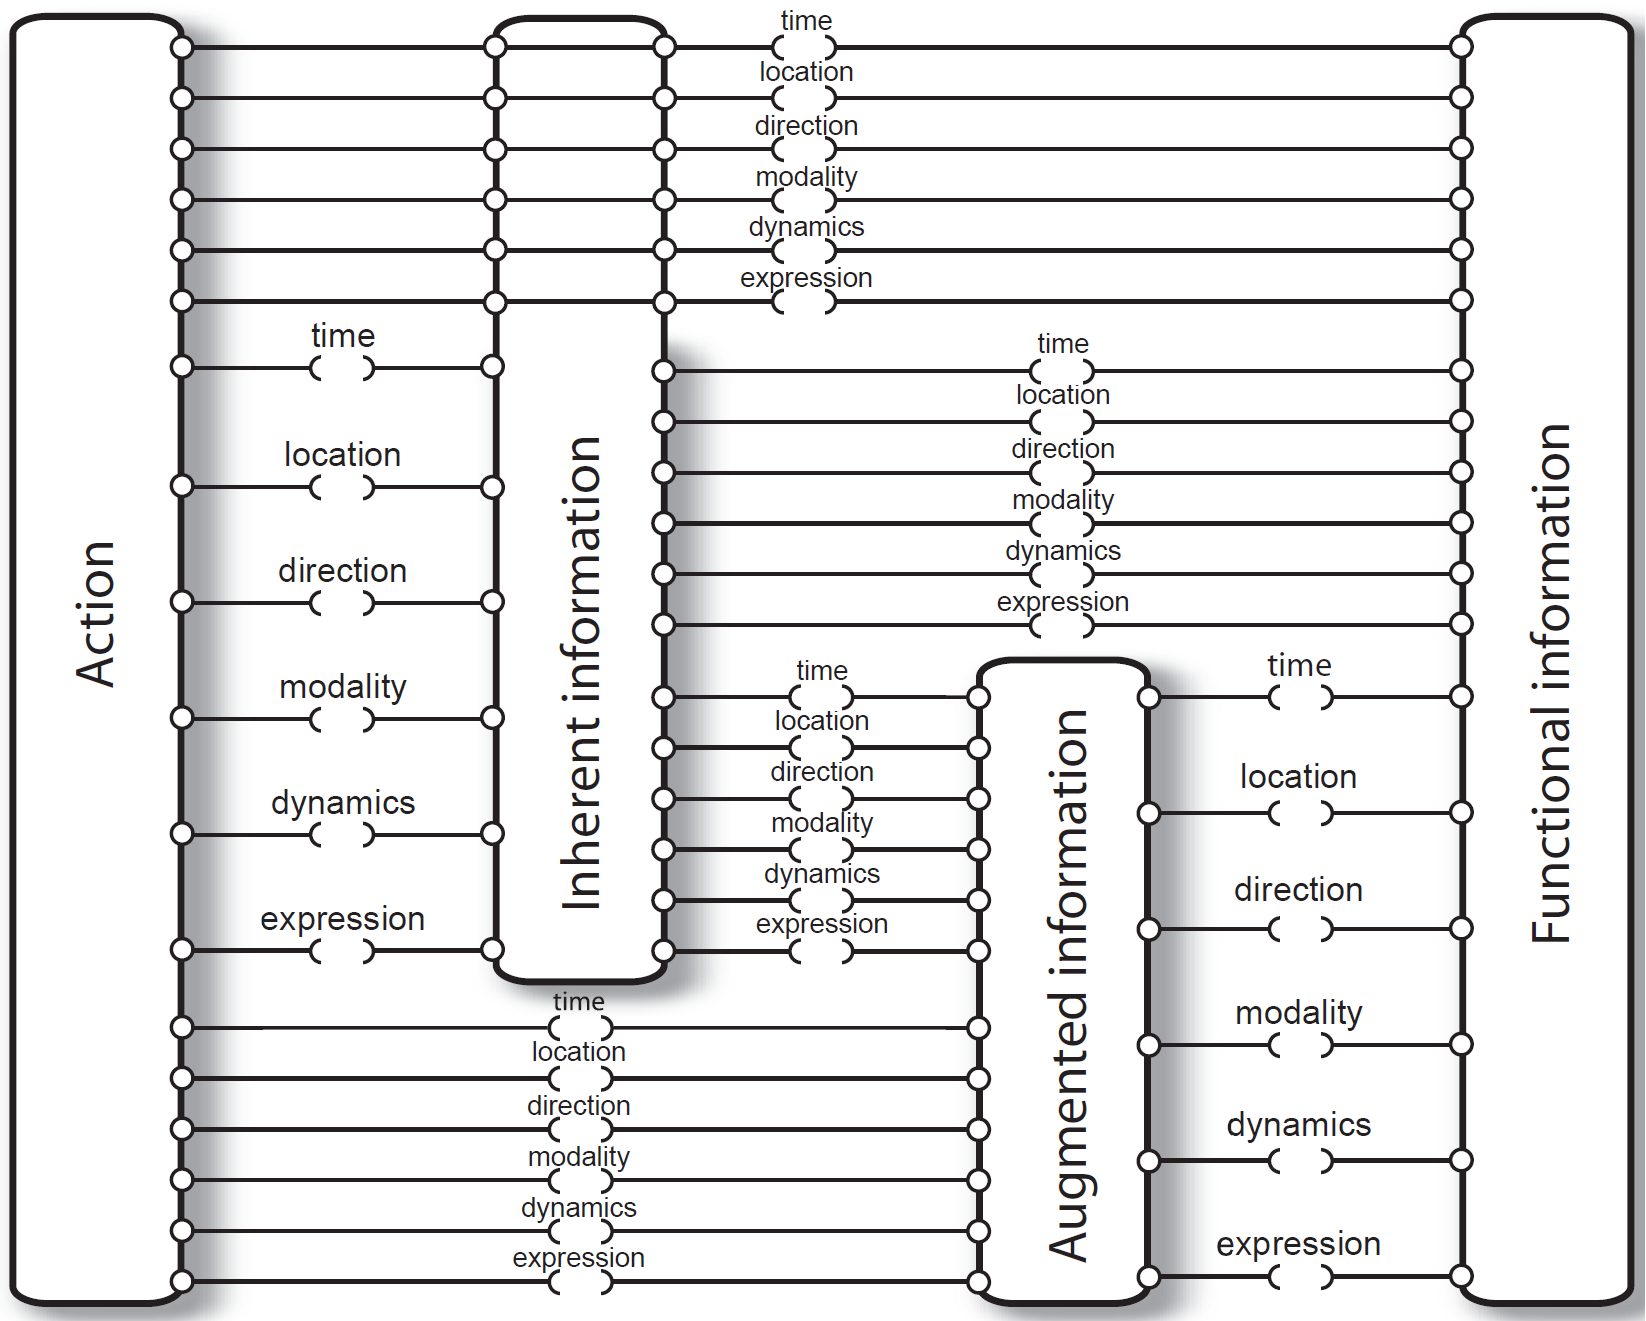
\includegraphics[width=\textwidth]{FroggerDefault}
  \caption{The Frogger Framework}
  \label{frogdef}
\end{figure}

From these two information directions (feedforward and feedback) with three subdivisions (functional, inherent and augmented) and six aspects to couple them on (time, location, direction, modality, dynamics and expression), \citeA{frogger} formulated a framework called the Frogger Framework (see figure \ref{frogdef}). The framework is a "[...] A schematic interpretation of all the different coupling possibilities between the functional information and the user’s action" \cite[p. 6]{frogger}. This schematic approach has a high amount of complexity and can perhaps be daunting and/or confusing to interpret, which could explain why others have chosen to simplify the model \cite{tangifrog} and why \citeA{transbehav}, who include Stephan Wensveen, see an altered and simplified model as "[...] more useful" \citeA[p. 22]{transbehav}. The altered and simplified version is also the version I will refer to henceforth (see figure \ref{frogalt}).

\begin{figure}[h]
  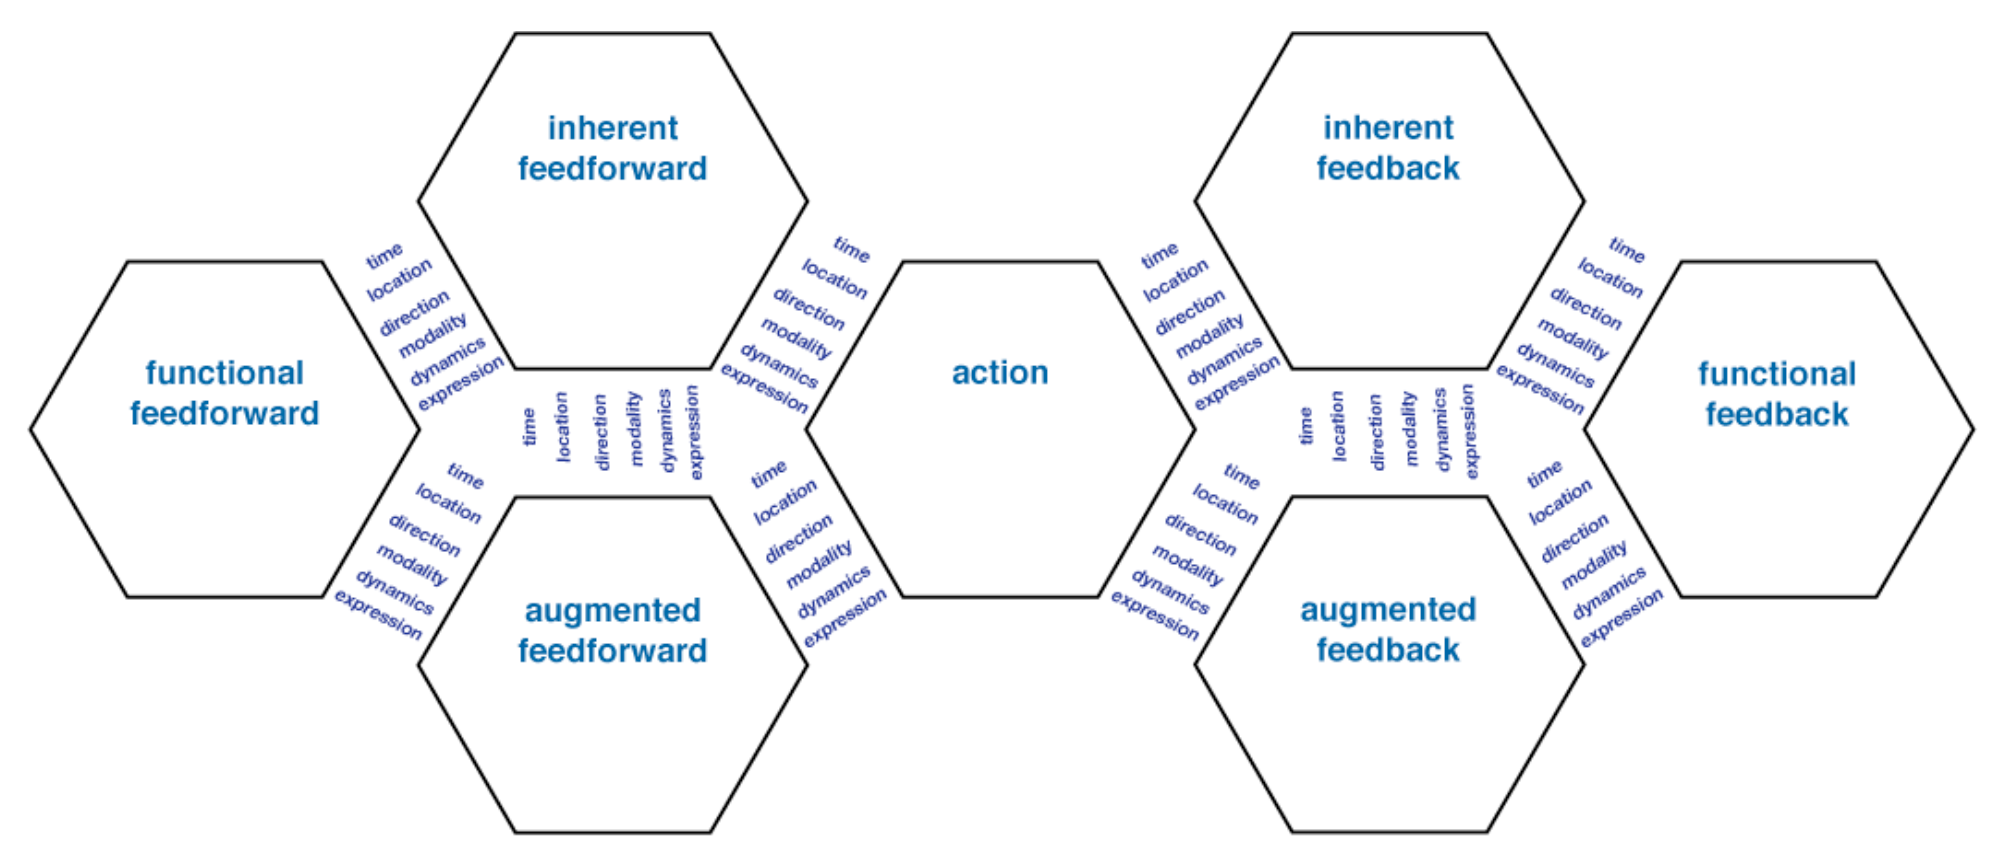
\includegraphics[width=\textwidth]{FroggerAlt}
  \caption{The Alternate Frogger Framework}
  \label{frogalt}
\end{figure}

\newpage


\chapter{Into the Void}
The Frogger Framework is not limited to electronic products: In \citeA{frogger} a mechanical product is analysed through the framework and in \citeA{transbehav} it is explained how a speed-skate experience is augmented as a result of using the framework. The limit of the framework is, perhaps purposefully, left unclear and its use is described as ``[...] to explore and create intuitive and aesthetic interaction'' \cite[p. 22]{transbehav}. Also, the initial formulation of feedforward and inherent feedback was done with the believe that meaning is of highest priority when designing: ``We argue that the creation of meaning in interaction is the key to making abstract concepts in consumer electronics accessible'' \cite[p. 2]{howdonald}. This concern of meaning is shared in the game design community: ``The goal of successful game design is the creation of meaningful play ''\cite[ch. 3, p. 3]{salen}. This conclusion is furthermore derived from \cite{huizinga}: ``In play there is something 'at play' which transcends the immediate needs of life and imparts meaning to the action. All play means something'' \cite[p. 1]{huizinga}. The difference between the approaches would be the use of the words \textit{interaction} and \textit{play}. With respect to differing and expansive definitions of what play is \cite{huizinga, sicartplay, salen}, I will regard it within the narrow scope of \textit{game play}, since I am operating in the field of game design. With this in mind, play can be regarded as a form of interaction: ``Game play is the formalized interaction that occurs when players follow the rules of a game and experience its system through play'' \cite[ch. 22, p. 3]{salen}.
Returning to the Frogger Framework: While the use of the framework may be unclear, it is clear that \citeA{frogger} operates within the field of \textit{embodied interaction} \cite{transbehav}. A possible intention for use of the framework can therefore be regarded as within the field of embodied interaction. Following previous notions, embodied interaction is also defined as being dependant on meaning \cite[p. 126]{dourish}. Although similar interests of meaning is prevalent in designing for games \cite{salen} and embodied interaction \cite{dourish}, an assumption that this would make the two correlative would be frail. So, a further analysis of embodied interaction is needed.

\section{Embodied Interaction}
Since embodied interaction relies heavily on the definition of \textit{embodiment}, I will shortly delve into the phenomenological tradition of Husserl, Heidegger and Merleau-Ponty, all of whom helped better the understanding of embodiment, as deduced by \citeA{dourish}. To ensure focus, I will adhere to \citeauthor{dourish}'s \citeyear{dourish} analysis of the three phenomenologists' work.

\paragraph{Husserl} Edmund Husserl was the first to define phenomenology. He found that current sciences of his time (1859-1938) was diverting from the physical everyday world with practical appliances into an idealised one which was not experienced but only theorised. A student of Franz Brentano, he embraced Brentano's notion of \textit{intentionality} which describes the relationship between the external reality and one's thoughts about it, i.e. the relationship between the chair you might be sitting on and your thoughts about it. Husserl imagined phenomenology as a rigorous science for examining the nature of intentionality. For this methodology he terms (1) \textit{noema} and (2) \textit{noesis} as being representations of (1) objects of intentionality and (2) our mental experiences of those objects. For this methodology to be rigorous Husserl defines the objective of phenomenology as to explain how we perceive objects as simply existing without question, i.e. explaining how a \textit{natural attitude} arises. This world of natural attitudes, Husserl later defines as the \textit{lebenswelt} (or \textit{life-world}). ``The life-world is the intersubjective, mundane world of background understandings and experiences of the world. It is the world of the natural attitude and of everyday experience'' \cite[p. 106]{dourish}. Husserl further argues that there is a parallelism in the objects one perceives and the act of perceiving them, as when an object is perceived, the act of perceiving it is also accepted. Otherwise, real-world perceptions would be indistinguishable from imaginings. This also means that fantasising or memorising can be individual experiences.

Lastly, Husserl makes a distinction between the immediate everyday sense-impressions and the recognition of the object in front of us as being a chair. The distinction is deduced as moving from the everyday world towards the formal world. Recognising the object as a chair is recognising the object's \textit{essence} \cite{dourish}.

\paragraph{Heidegger} Martin Heidegger, a student of Edmund Husserl, departs from Husserl's mentalistic approach. While Husserl adopted Descartes' \textit{cartesian dualism}, which dictates that ``[...] we 'occupy' two different and separate worlds, the world of physical reality and the world of mental experience'' \cite[p. 107]{dourish}, Heidegger was concerned with the lack of attention from Husserl and his peers to the world of physical reality and argued that being comes before thinking: In order to think one has to be. Therefore, Heidegger rejected this dualism and argued that being and thinking is intertwined and cannot be separate from the other. Heidegger's development of phenomenology was roughly a shift from an epistemological approach to an ontological one, i.e. instead of focusing on how we obtain knowledge of the world, we should focus on how the world presents itself to us: ``From his perspective, the meaningfulness of everyday experience lies not in the head, but in the world'' \cite[p. 107]{dourish}.

Intentionality, as Husserl defined it, was for Heidegger too passive. For Heidegger, intentionality is not only concerned with perception, but is of a practical nature. It is based on our concern for utilisation and how we can manipulate something, i.e. a chair is a chair because we can sit on it. This meaning, according to Heidegger, is already existing in the world and is only interpreted by us, and this interpretation is what Heidegger is concerned with.

From Heidegger's work, two concepts are of most importance for the context of this thesis: (1) \textit{Dasein}, (or \textit{being-in-the-world}) and (2) \textit{das Zeug} (or \textit{equipment/tools}) \cite{heidegger}.
(1) Dasein explains the experience of being in the world, and sometimes as exemplified in an entity experiencing the world as we do. Specifically it is the relation between the being and the world, which in turn are inseparable. For Heidegger, Dasein is active and with a practical approach. The world is perceived as objects to be used or manipulated, but also a medium through which to act. More concretely, Dasein often perceives the world with the intention of accomplishing goals.
(2) For Dasein to accomplish these goals there are Zeug. Heidegger sums up Zeug as being something in-order-to, meaning that the Zeug is always linked to a task. While being linked to a task, Zeug is also linked to other Zeug in ways that it ``[...] relies upon, works with, suggests, is similar or dissimilar to, or is otherwise related to other equipment'' \cite[p. 109]{dourish}. Heidegger's Zeug also plays a particular important role within the context of this thesis with his distinction between \textit{zuhanden} (ready-to-hand) and \textit{vorhanden} (present-at-hand) \cite{heidegger}. To explain the distinction I will exemplify it with you considering a regular pencil as the Zeug. You pick it up and position it between your fingers. As you align the pencil to your preference, the pencil is vorhanden: You have to account for weight and balance it, hence its presence is obvious to you. When you have positioned the pencil you start drawing. Quickly, the pencil is absorbed into your being, it becomes zuhanden: You no longer actively consider the weight or balance of the pencil, but instead you act through the pencil producing pencil strokes. In a sense, you have become a being capable of drawing, instead of a being holding a pencil. To elaborate, Heidegger suggest that the pencil is only objectively present to us because of its possibility of becoming vorhanden, and as soon as it becomes zuhanden it withdraws from the world as an individual object, and is instead incorporated in the being. Should you perhaps find this absurd and check your hand to affirm that the pencil is indeed still there, you will find that the pencil has returned to the state of vorhanden, and is therefore present independent of your being \cite{dourish}.

\paragraph{Merleau-Ponty} Maurice Merleau-Ponty was particularly concerned with the body's role in perception, and his work is central when discussing embodiment. For Merleau-Ponty the body was the key to bridging the work of Husserl and Heidegger, which he thought was addressing the same problems but from different perspectives \cite{ponty}. Merleau-Ponty argued that the body can be considered as more than just psychophysical: That, in relation to the senses of the body, it can be considered the medium through which the external reality is perceived. The body therefore is what connects Husserl's ideas of perception and Heidegger's concern with being-in-the-world (the external reality). This, in turn, means that the body is both subject and object: The perceiver's body being subject, and the perceived body as being object.

This addition of a body as a mediation between Husserl and Heidegger makes the importance of what embodiment means clear. For this, Merleau-Ponty offers three definitions: ``The first is the physical embodiment of a human subject, with legs and arms, and of a certain size and shape; the second is the set of bodily skills and situational responses that we have developed; and the third is the cultural 'skills', abilities, and understandings that we responsively gain from the cultural world in which we are embedded'' \cite[p. 114]{dourish}.
\\
Building on these four perspectives on embodiment, \citeA{dourish} draws a definition: ``Embodiment is the property of our engagement with the world that allows us to make it meaningful'' \cite[p. 126]{dourish}. With this definition he then goes on to define embodied interaction: ``Embodied Interaction is the creation, manipulation, and sharing of meaning through engaged interaction with artifacts'' \cite[p. 126]{dourish}.

Then, I return to the question of whether or not game design can be to design for embodied interaction. \citeA{dourish} believes that this is not the case: ``Even in an immersive virtual-reality environment, users are disconnected observers of a world they do not inhabit directly. They peer out at it, figure out what’s going on, decide on some course of action, and enact it through the narrow interface of the keyboard or the data-glove, carefully monitoring the result to see if it turns out the way they expected. Our experience in the everyday world is not of that sort'' \cite[p. 102]{dourish}. \citeA{dourish} argues that video games uses the physical world as a metaphor for interaction to convey meaning to the player, and that this is not compatible with the embodied interaction we encounter in the real world. While not directly disagreeing, I will provide a perhaps more nuanced argument on how talking about embodiment in video games can be constructive.

\section{Embodiment in Video Games}
As previously discussed, intentionality describes the relationship between action and meaning, i.e. the intention of an action. Now, imagine playing a video game with a 3D simulated world wherein you come upon a challenge of pressing a button to open a door. You manoeuvre your avatar up to the button and press it, with the intention of opening the door. For the door to be intentionally opened by you, a chain of couplings \cite{dourish} need to be made: First the input of your finger on the relevant key of the device running the game, then the in-game agent's push of the button and finally the door opening. You do not act directly on the door, but your intention is still directed towards the door.

This notion of coupling is not dissimilar to the one discussed in \citeA{frogger} albeit this definition from \citeA{dourish} is not confined to the six aspects of time, location, direction, dynamics, modality and expression. Instead, \citeA{dourish} argues that when you experience a tool as Heidegger's zuhanden, the tool and you are coupled. Furthermore, as is clear from the previous example, the coupling can cover distances and thereby be remote from a local action, a fact that is also addressed in \citeA{frogger} when discussing coupling on the aspect of location: ``One can argue that the location of your fingers and your hand do not coincide with the cut of the paper. But because the scissors become an extension of your hand when cutting the paper (Heidegger’s concept of ‘ready-to-hand’ or ‘zuhanden’), you act through the scissors at the same location as the paper is being cut'' \cite[p. 2]{frogger}. So, when a tool becomes zuhanden, local actions can have remote intentions.

Combining this observation with the fact that couplings can also be made with abstract representations \cite{dourish}, there is grounds to explore whether or not input devices for video games can be considered tools able to become zuhanden. Video game controllers have a tendency to be more complex than e.g. the pen from a previous example, and if you were to hand such a controller to a relative who had never used such a device before, there would be little chance that the controller would become zuhanden for him or her in the course of an afternoon. How, if possible, does such a device become zuhanden?

\subsection{Internalisation}
\citeA{calleja} argues that \textit{involvement} is the key prerequisite to presence in video games. On the topic of zuhanden, \citeauthor{calleja}'s \citeyear{calleja} definition of in-game kinaesthetic involvement is of clear relevance. Kinaesthetic involvement relates to the way a game translates input from the player to the allowed \textit{agency} within the game context through an \textit{avatar} or \textit{miniatures} \cite{calleja}. Agency within games pertains to the effect the player is able to assert in the game context. It is not referring to any intentions the player may have, but is instead the ability to perform intention-carrying actions. The avatar and the miniature are one or more entities that carry out the actions dictated by the player. The distinction between the two is that the avatar works as a representation of the player in the game world and is operated independently. Kinaesthetic involvement, then, is the involvement required to control an avatar or miniature \cite{calleja}.

The varying amount of conscious effort kinaesthetic involvement may take up is dependant on the player's attention. A new player as an example may require a large amount of attention to the controls, and as she progress, less attention is needed, in turn minimising the effort required for kinaesthetic involvement. \citeA{calleja} describes the state of minimal or no attention towards involvement as the involvement being \textit{internalised}. This diminishing attention is similar, if not identical, to Heidegger's notion of equipment withdrawing from the world to become zuhanden: ``The internalization of kinesthetic involvement describes a situation in which the controls are learned to such a degree that the on-screen movement of avatars and miniatures feels unmediated'' \cite[p. 68]{calleja} and ``[...] players must be able to 'think with their fingers' to the point at which the player feels like an extension of the game or the game feels like and extension of the player'' (\citeA{morris} in \citeA[p. 68]{calleja}). So, admitting that the phenomenological discussion on the matter can be much more nuanced and complex, for the sake of keeping focus, I will from this point forward consider game controls on the same level as Heidegger's equipment, thereby also considering them as capable of becoming zuhanden.

Just as \citeA{dourish} then describes the embodied interaction of acting on a classical WIMP (windows, icons, menus, pointers) interface through coupling, I might do the same with video games and because of this alignment I would be able to use the Frogger Framework \cite{frogger}. This would, however, limit the intricate detail that can be present in e.g. 3D or VR video games. It is obvious that this detail is present in the game world, so addressing it would be paramount for my framework. How, then, to address this detail will be the topic of the next section.

\subsection{Ludic Subjectivity}
The notion of kinaesthetic involvement is, as discussed, part of the more general term of involvement and as internalised involvement intensifies and the six dimensions (kinaesthetic, spatial, shared, narrative, affective and ludic) start to blend, the experience of the player moves towards an experience of \textit{incorporation} \cite{calleja}. Incorporation is thusly defined as ``[...] the absorption of a virtual environment into consciousness, yielding a sense of habitation, which is supported by the systemically upheld embodiment of the player in a single location, as represented by the avatar'' \cite[p. 169]{calleja}.

\citeA{vellashort} believes that this embodiment of the player in the game world can be described as the \textit{embodied ludic subject} which implies a point within this world from which the player can relate: ``[...] the player’s incorporation in the form of the playable figure grants her a spatial standpoint within the gameworld – an origo or point of origin to which deictic terms like ‘here,’ ‘there,’ ‘ahead’ or ‘to the left’ relate'' \cite[p. 4]{vellashort}. This is in congruence with the notion of spatial involvement from \citeA{calleja}, which, like kinaesthetic involvement, implies a necessity of internalisation before the player can be incorporated. This means that an incorporated player inhabits a point within the game world through an avatar or miniature from which the player relates this internal environment including visual and auditory information.

Following the definition of embodiment, a being's capability to act upon the world is central \cite{ponty}. \citeA{vella} argues that this capability is determined by the representation of the player within the game world. The player's capability is thus defined and limited by e.g. an avatar. This sense of what 'I can' and 'cannot' do is what shapes the world around us. Remembering \citeA{heidegger}, the objects of the world is only present to us in the way that they are able to be acted upon by us. The fact that we, when stumped in solving a challenge in a video game, can counter 'I cannot make that jump' to a passer-by suggesting that we 'just jump', bolster the argument that what is occurring on a mental level of the incorporated player is not a 'I think that my avatar is able to' but an 'I can' \cite{vellashort}. Furthermore, just as embodiment requires an ability to act upon the world it also requires the reverse: For the world to act upon the body \cite{ponty}. \citeA{vella} terms games' ability to act upon the embodied ludic subject as \textit{passion}, but not in the word's popular definition, but as the inverse of the word \textit{action} \cite{vella}. The term concerns the way the game world or agents in it can act upon the ludic subject and in turn how the player experiences this possibility. When I, for example, sneak around in \citeA{metalgear} I embody the fear of being discovered.

\section*{Summing Up}
Returning then, to the misjudgement of \citeA{dourish}: ``Even in an immersive virtual-reality environment, users are disconnected observers of a world they do not inhabit directly. They peer out at it, figure out what’s going on, decide on some course of action, and enact it through the narrow interface of the keyboard or the data-glove, carefully monitoring the result to see if it turns out the way they expected. Our experience in the everyday world is not of that sort'' \cite[p. 102]{dourish}. From this citation I can extract three arguments: (1) virtual game environments cannot be inhabited, (2) actions within a game world are mediated and require high attention and (3) experiences in the everyday world are dissimilar to the ones in a game world.

Through the research presented in this thesis I deem there to be substantial evidence countering these arguments. \citeauthor{dourish}'s \citeyear{dourish} first argument of virtual environments being uninhabitable I have provided counterarguments to by referencing \citeauthor{vella}'s \citeyear{vella} notion that a player's incorporation \cite{calleja} establishes an embodied ludic subject with a spatial point within the game world from where the player inhabits said world.

The second argument that actions in the game world are mediated and necessitates high attention I have provided counterarguments to by referencing \citeauthor{calleja}'s \citeyear{calleja} concept of involvement (especially kinaesthetic involvement) where a player's continuous involvement leads to an internalisation of controls which minimises the required attention of the player. Additionally, \citeauthor{vella}'s \citeyear{vella} arguments for embodied ludic subjectivity opposes the idea that games are mediated in the context of embodiment.

The third argument can thus be said to be misdirected since it can now be argued that the game world is incorporated into the player's lebenswelt and the playable figure becomes an extension of the player, in other words part of the player's \textit{body schema} \cite{vellashort}, which \citeA{haans} defines as the following: ``The body schema can, thus, best be described as a dynamic distributed network of procedures aimed at guiding behavior'' \cite[p. 213]{haans}.




\section{Framework}
Through the discussed theory I have formulated a framework (see figure \ref{framework}) which takes influence from the Frogger Framework \cite{frogger} and is adapted it into a game design or game analysis context. The notions of augmented, inherent and functional information is transferred as they were aswell as the six aspects of time, location, direction, dynamics, modality and expression. A few aesthetic distinctions has been made to the visual representation of the framework to improve readability and functionality, as an example the horizontal division represents the division between feedforward on top and feedback at the bottom. This is done to avoid confusion that may arise when trying to discern if a coupling is through feedforward or feedback, which has arisen in other adaptations of the Frogger Framework \cite{tangifrog}. What follows here, however, addresses the changes made to the framework itself and not the aesthetic changes of a model.

\begin{figure}
  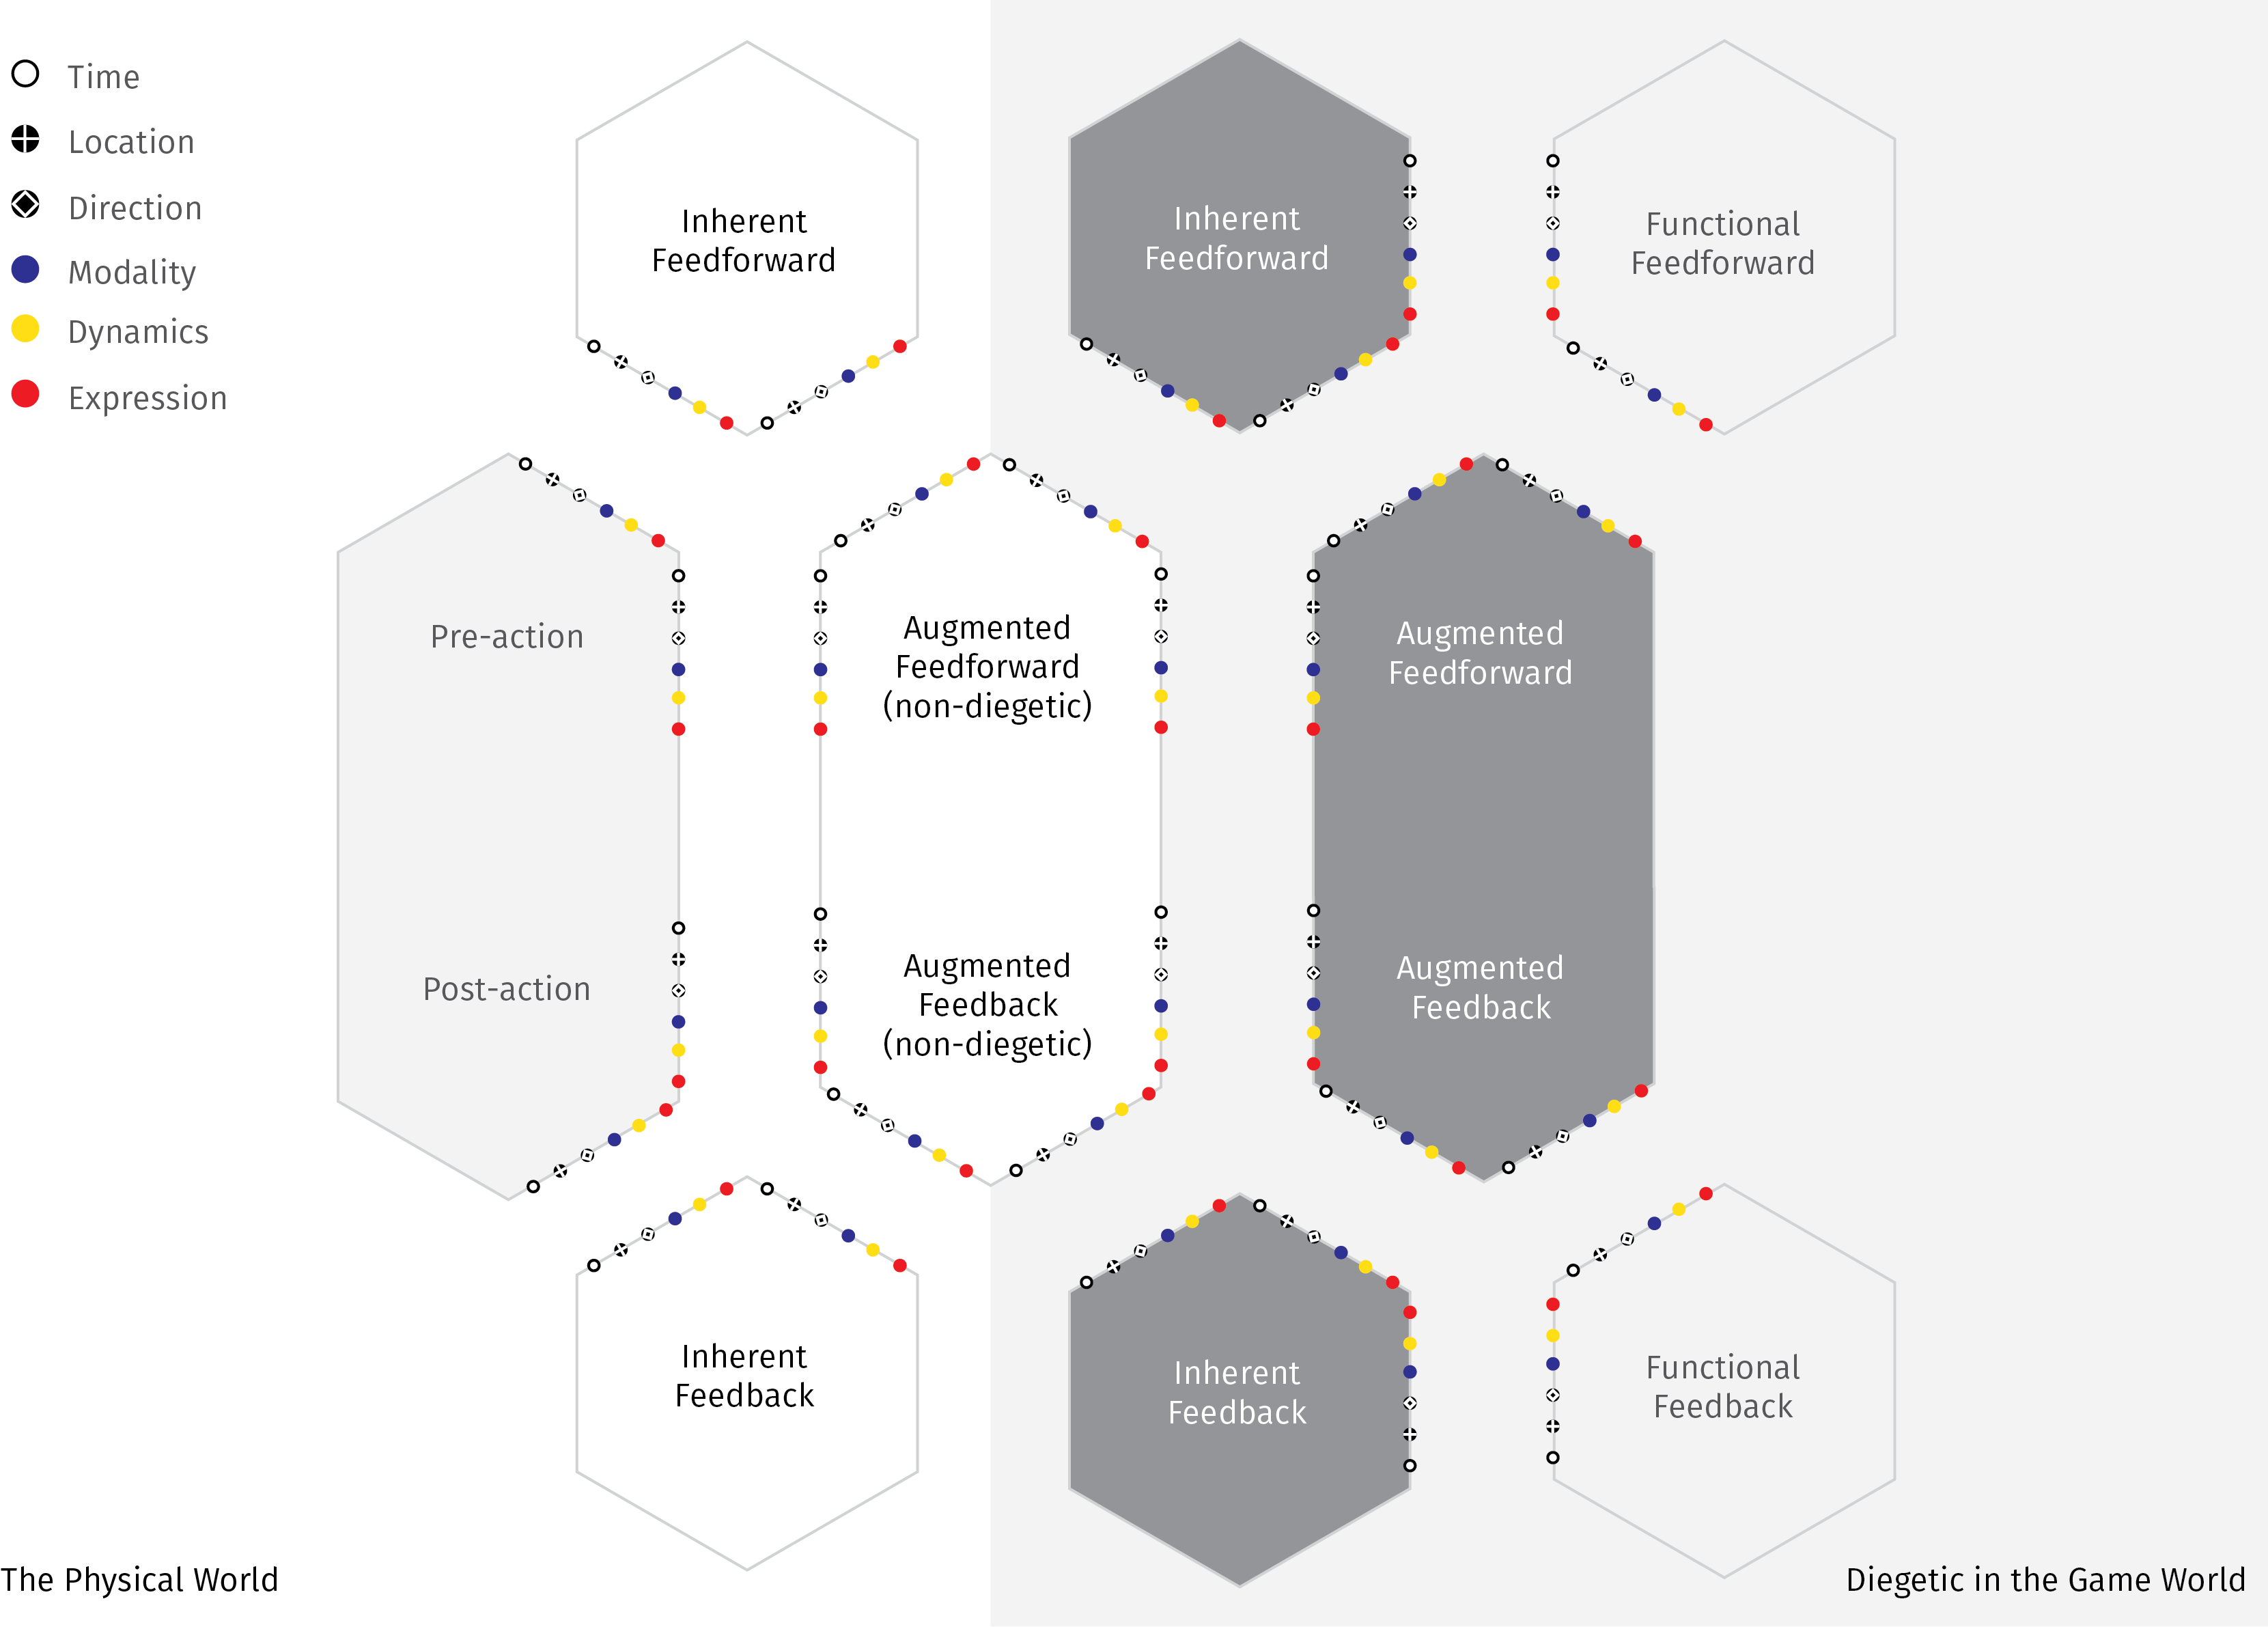
\includegraphics[width=\textwidth]{Framework}
  \caption{The Framework}
  \label{framework}
\end{figure}

\subsection{The Ludic Heterocosm}
The framework is divided on two axes. The horizontal, as discussed above, separates feedback from feedforward. The vertical division represents the division between the physical world and the game world. All things only existing in the physical world operates on the left side, and everything diegetic to the game world, i.e. what can be seen, heard, felt, tasted, smelled, touched, etc. by an entity in the game world operates on the game world side \cite{bordwell}. \citeA{vella} describes this world as the \textit{ludic heterocosm}. What is important to note about the ludic heterocosm is that it extends beyond what is visible on the screen at any one moment. It is an imagined world created in the player's mind. As an example, when meeting a travelling salesman of the Khajiit race in \textit{The Elder Scrolls V: Skyrim} \cite{skyrim}, the player may include the salesman's homeland of Elsweyr into her ludic heterocosm even though it is never visited in the game.

Even though both the game world and the physical world can be said to operate within Husserl's lebenswelt, the distinction has been made to address the detail that exists on both sides of the screen mediating a video game. On the physical side it can be the button layout of a Game Boy and on the game side it can be the shape of the incoming tetromino moving from top to bottom in \textit{Tetris} \cite{tetris}. With inherent and augmented information in the physical world being identical to the formulation in the Frogger Framework, what then becomes relevant to discuss is how augmented and inherent information is experienced in the ludic heterocosm.

The Frogger Framework definition uses concrete delimited design examples like scissors and a DVD-player \cite{frogger}, but has also been used to improve experiences like the Augmented Speed-skate Experience \cite{transbehav}. This is indicative of how the entire interaction experience is included in the framework, which is also imperative in a video game context. When playing a video game, all the models and the environment within the game world is designed with intent. The developers behind the particular game has made decisions on all levels of what is presented to the player. Some, more deliberate than others, yet all of them stem from a decision. This means, among other things, that augmented information in the game world can originate from unconventional places compared to the physical world because of the delimited context the developers are able to control. One could argue that a semantic constraint is able to involve the entire game world. For example, when I enter a dungeon in \textit{The Legend of Zelda: A Link to the Past} \cite{linktothepast} I trust that most signifiers and perceivable affordances within the dungeon are there to guide me towards attaining the key item and defeating the boss. In the physical world there is noise. Experiences in the physical world are not granted the benefits and hindrances from being inside the vacuum of a designed simulation, game worlds are. Therefore, designing for \textit{usability} in level design, i.e. using level design as a method for teaching, can be an opportunity for strengthening a coupling through augmented information \cite{totten}. This is, however, not to say that augmented information in the game world is different from augmented information in the physical world, but merely to address the possibility of uncommon expressions of augmented information in the game world.

Inherent information in the game world is not inherent from the action of the player but instead from the action of the playable figure. In \textit{The Legend of Zelda: Skyward Sword} \cite{skyward} the direction a sword is swung is critical. Some directions will result in negating the desired effect or even losing health points. How the correct direction is communicated then, is through inherent information. As an example, the enemy type called Deku Baba, will only take damage from a sword if the sword is swung on the same axis as its jaw is opened (see figure \ref{dekubaba}). The enemy model effectively communicates this inherent information because it informs the actions that are possible (slicing) and how to carry it out (slicing directions).

\begin{figure}[h]
  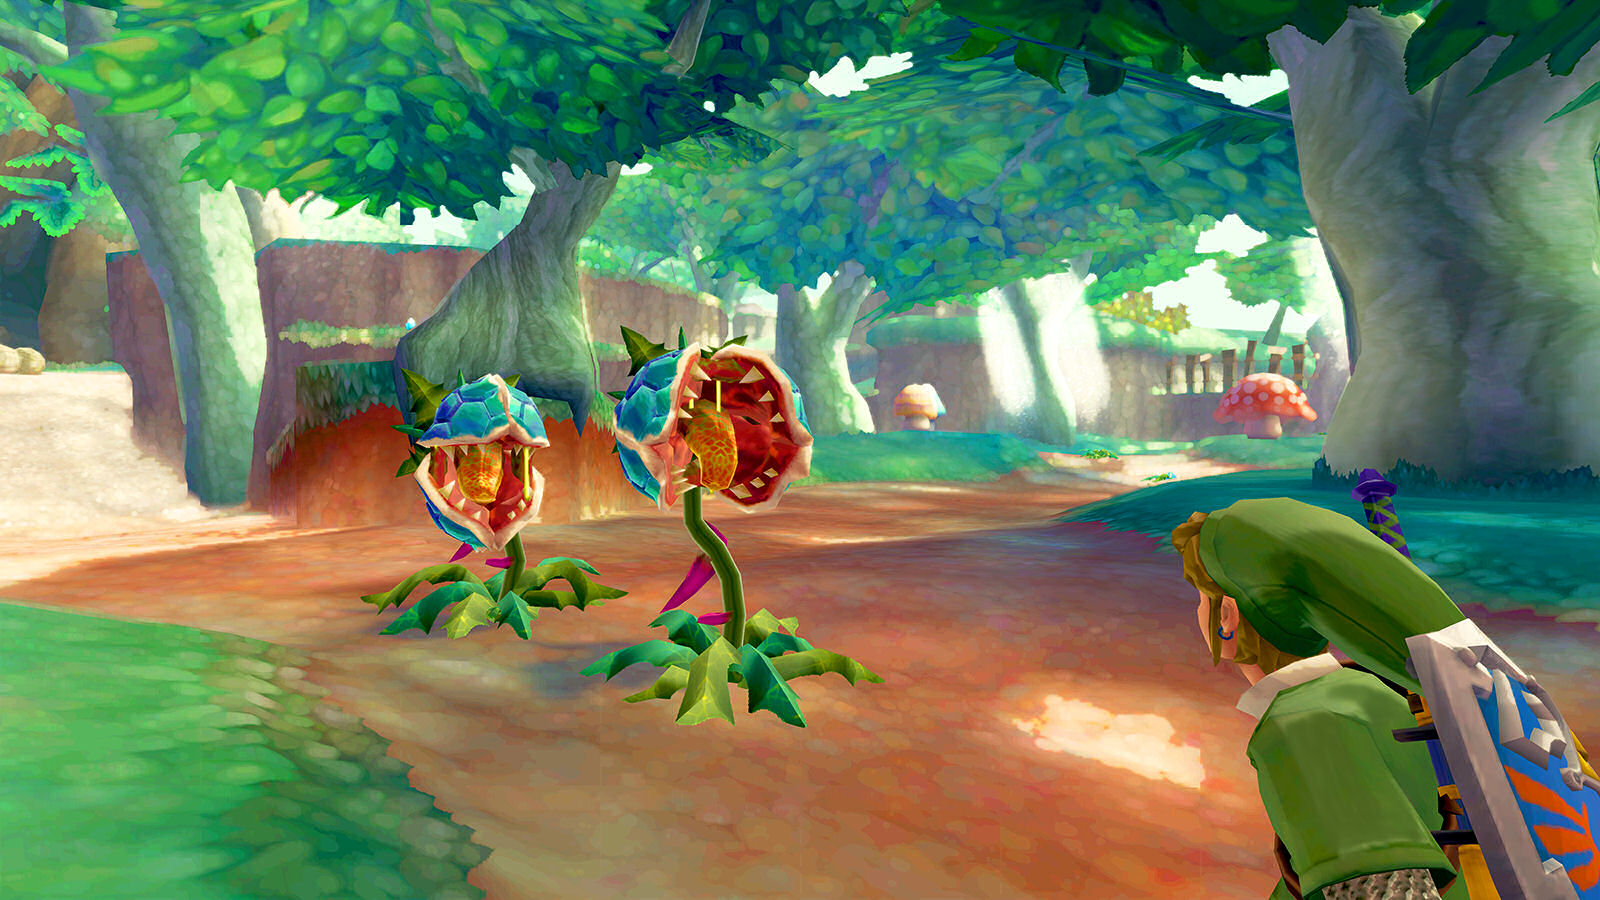
\includegraphics[width=\textwidth]{DekuBaba}
  \caption{The enemy type Deku Baba from The Legend of Zelda: Skyward Sword, will only take damage from a sword if the sword is swung on the same axis as its jaw is opened}
  \label{dekubaba}
\end{figure}

\subsection{Applying the Framework}
It is of great consideration when I make the distinction on the aspect of diegesis. A head-up display (HUD) is, as an example, sometimes not diegetic to the game world and, as a consequence, not existing for any agent within the game world. It can thus be said to provide meaning for the actions of the player and not the ludic subject, and therefore a HUD would usually be influential in regards to the augmented information of the physical world. What the framework's distinction then is attempting to mirror is the notion of involvement \citeA{calleja}. It can, however, not be said to integrate all six dimensions of involvement. The dimensions relevant to this framework is spatial involvement and kinaesthetic involvement. Spatial involvement is relevant because of the spatial point that is inhabited in the game world, and from this point the framework's aspects of location and direction relates. Kinaesthetic involvement is relevant because it is integral to a sense of control for the player and the fact that a close coupling on the six aspects of this framework leads to intuitive interaction \cite{frogger} should also lead to a higher degree of internalisation on the dimension of kinaesthetic involvement since it requires less attention as is also argued by \cite{calleja}:
\begin{quote}
  In the kinesthetic involvement dimension, conscious attention is generally dedicated to learning the controls of the game during a player’s early sessions of playing. This includes following on-screen instructions relating to avatar control or looking up and reassigning keys and buttons to the desired controls and then testing how these feel in the game. As players find the control setup that feels most intuitive to them or get used to the one supplied by the game, their conscious attention moves away from the basic controls to other aspects of the game. [...] In such cases, we can say that the player has 'internalized' the controls: she has reached a level of kinesthetic involvement that requires little or no conscious effort \cite[p. 45]{calleja}.
\end{quote}
Keeping in mind that any practical use of the framework in regards to design has the goal of improving intuitiveness of interaction, this means that the optimal use cases of the framework is when the player has not internalised the controls, since an internalisation would mean that the controls have indeed already become intuitive. Because of this, a relevant use case would be when a game introduces a \textit{game mechanic}, since the player would not have internalised the controls of the new mechanic at the time of the introduction, given that it is the first time playing.

Game mechanics can be defined in various ways, but for the context of this framework, the one offered by \citeA{sicartmechanic} is fitting: ``Game mechanics are methods invoked by agents, designed for interaction with the game state'' \cite{sicartmechanic}. \citeA{sicartmechanic} is borrowing from the terminology used in the field of object-oriented programming when he uses the word 'methods', but to clarify, he argues that these methods can be considered as verbs describing the action that is possible to be utilised by an agent. As an example, the player is able to ride a horse in \textit{The Witcher 3: Wild Hunt} \cite{witcher}, which when considering methods as verbs makes 'riding' a game mechanic. In \textit{The Witcher 3: Wild Hunt} \cite{witcher}, however, riding could be said to be comprised of several mechanics such as 'speeding', 'slowing' and 'halting'. \citeA{sicartmechanic} categorises these inclusive game mechanics as \textit{compound game mechanics}. In regards to granularity and the framework, the higher the detail, the less the confusion. If a compound game mechanic were to be described in the framework, the complexity created by the different sub-mechanics would in many cases lead to contradiction on the six aspects and the three types of information. A concern that is also addressed by \citeA{dourish} in regards to the complexity of computer systems:
\begin{quote}
  The consequence, then, is that there are very many different levels of description that could be used to describe my activity at any given moment. Some, perhaps, are ready-to-hand and some present-at-hand at the same time; my orientation toward them each will change. For instance, sometimes as I move the mouse, the mouse itself is the focus of my attention; some-times I am directed instead toward the cursor that it controls on the screen; at other times, I am directed toward the button I want to push, the e-mail message I want to send, or the lunch engagement I am trying to make \cite[p. 140]{dourish}
\end{quote}
Therefore, when designing or analysing the horse interaction in \textit{The Witcher 3: Wild Hunt} \cite{witcher}, the mechanic to logically be addressed first is not 'riding' but 'mounting'. \\
Then, as discussed earlier, the framework should be used in the situation of introducing a player to a new game mechanic. This means that for the framework to be used, there needs to exist a game mechanic. It is therefore, not especially relevant in the initial formulation of a game mechanic. Where it does become relevant, is in the iteration thereafter. Examples of how this can be done follows later.

\subsection{Examples}
Game examples Witcher 3 horse riding

Zelda Skyward Sword and the enemies showing how to strike (direction).

WarioWare telephone

Something about symbolic, mimetic and symbiotic control being clearly visible on the physical world part of the model \cite[p. 64]{calleja}


\chapter{A Method for Application}
\textit{``I hate portals''} \\
\rightline{Geralt of Rivia} \\
\rightline{The Withcer 3: Wild Hunt \cite{witcher}}

\section{A Delegation of Effort}
When having used the framework for analysis, it is clear that use in a design context would not be constructive, since the complexity necessitates a high degree of absorption and, most importantly, loads of time. Therefore, for the creation of a practical method, I decided to delegate the effort into two parts taking place during well-known processes in game development: playtesting and ideation. To test the effectiveness of the proposed method, I gathered a group of experienced game developers who, importantly, have not undertaken the same education specialisation as me, which assisted the developing of a universal method, and avoided the method specifying into a narrow school of thought. Another benefit of the test group was that they had previously worked on games together which limited the amount of noise arising from not knowing each others' approaches to game development, and assuring a solid baseline for comparison to previous development situations. The testing was separated into three phases corresponding to the two processes of playtesting and ideation. The first phase consisted of a playtesting situation with a prototype video game made by me specifically for the test following the ideas presented in \citeA{prototype}. I, then, acted as the interviewer and each group member acted in turn as the playtester. The second phase consisted of the group being presented with a drawn model on a whiteboard representing the simplified framework and the data I had gathered from the playtest. The third and last phase consisted of a semi-structured focus group interview \cite{cresswell} where the participants had a chance to discuss their impressions. The method for gathering qualitative data was chosen to be a focus group. This method was chosen because it is effective in gathering data from a group of respondents \cite{cresswell}, and since the target group for the method is a game development team, this was deemed suitable.

The main goal of the prototype video game was for it to be used as a tool for evaluating the proposed method, so the most important aspect was identified as the prototype aspiring to be as original as possible. The intent of this was to disconnect previous experiences the test participants might have had if the prototype had been similar to a game they had played previously, thereby optimistically limiting unknown variables in the evaluation. Realising that creating something original is a perilous task, an emphasis was simply put on implementing as few as possible conventional game mechanics such as using the W, A, S and D key for movement. Consequently, movement in the prototype is controlled by a mouse-wheel with the playable figure also resembling this wheel (see figure \ref{prototype}). The prototype consists of three minor challenges to ground the player in the control scheme and one integral kinaesthetic challenge as the focus of the test. This kinaesthetic challenge can be seen in figure \ref{prototype}. It consists of two doorways, one from which the player enters and the other through which the player needs to exit. Between the two doorways is a lowered area creating a gap between the two which makes travelling from one doorway directly to the other impossible since the playable figure cannot inherently move vertically. Leaning on the pathway leading into the room is a large barrel oriented horizontally which is suspended off the lower ground by a round beam going through the barrel's centre. The beam is held up by its extremities lying in two grooves in the walls perpendicular to the doorways. Lastly, the room is sloping toward the entrance making the entrance level slightly lower than the exit. The intended strategy to get to the other side is then to position the playable figure, a wheel, on top of the barrel and then use the weight of the wheel to rotate the barrel, which rotates the beam that progresses everything forward towards the exit where the player can climb off the barrel and exit.

\begin{wrapfigure}{i}{0.6\textwidth}
  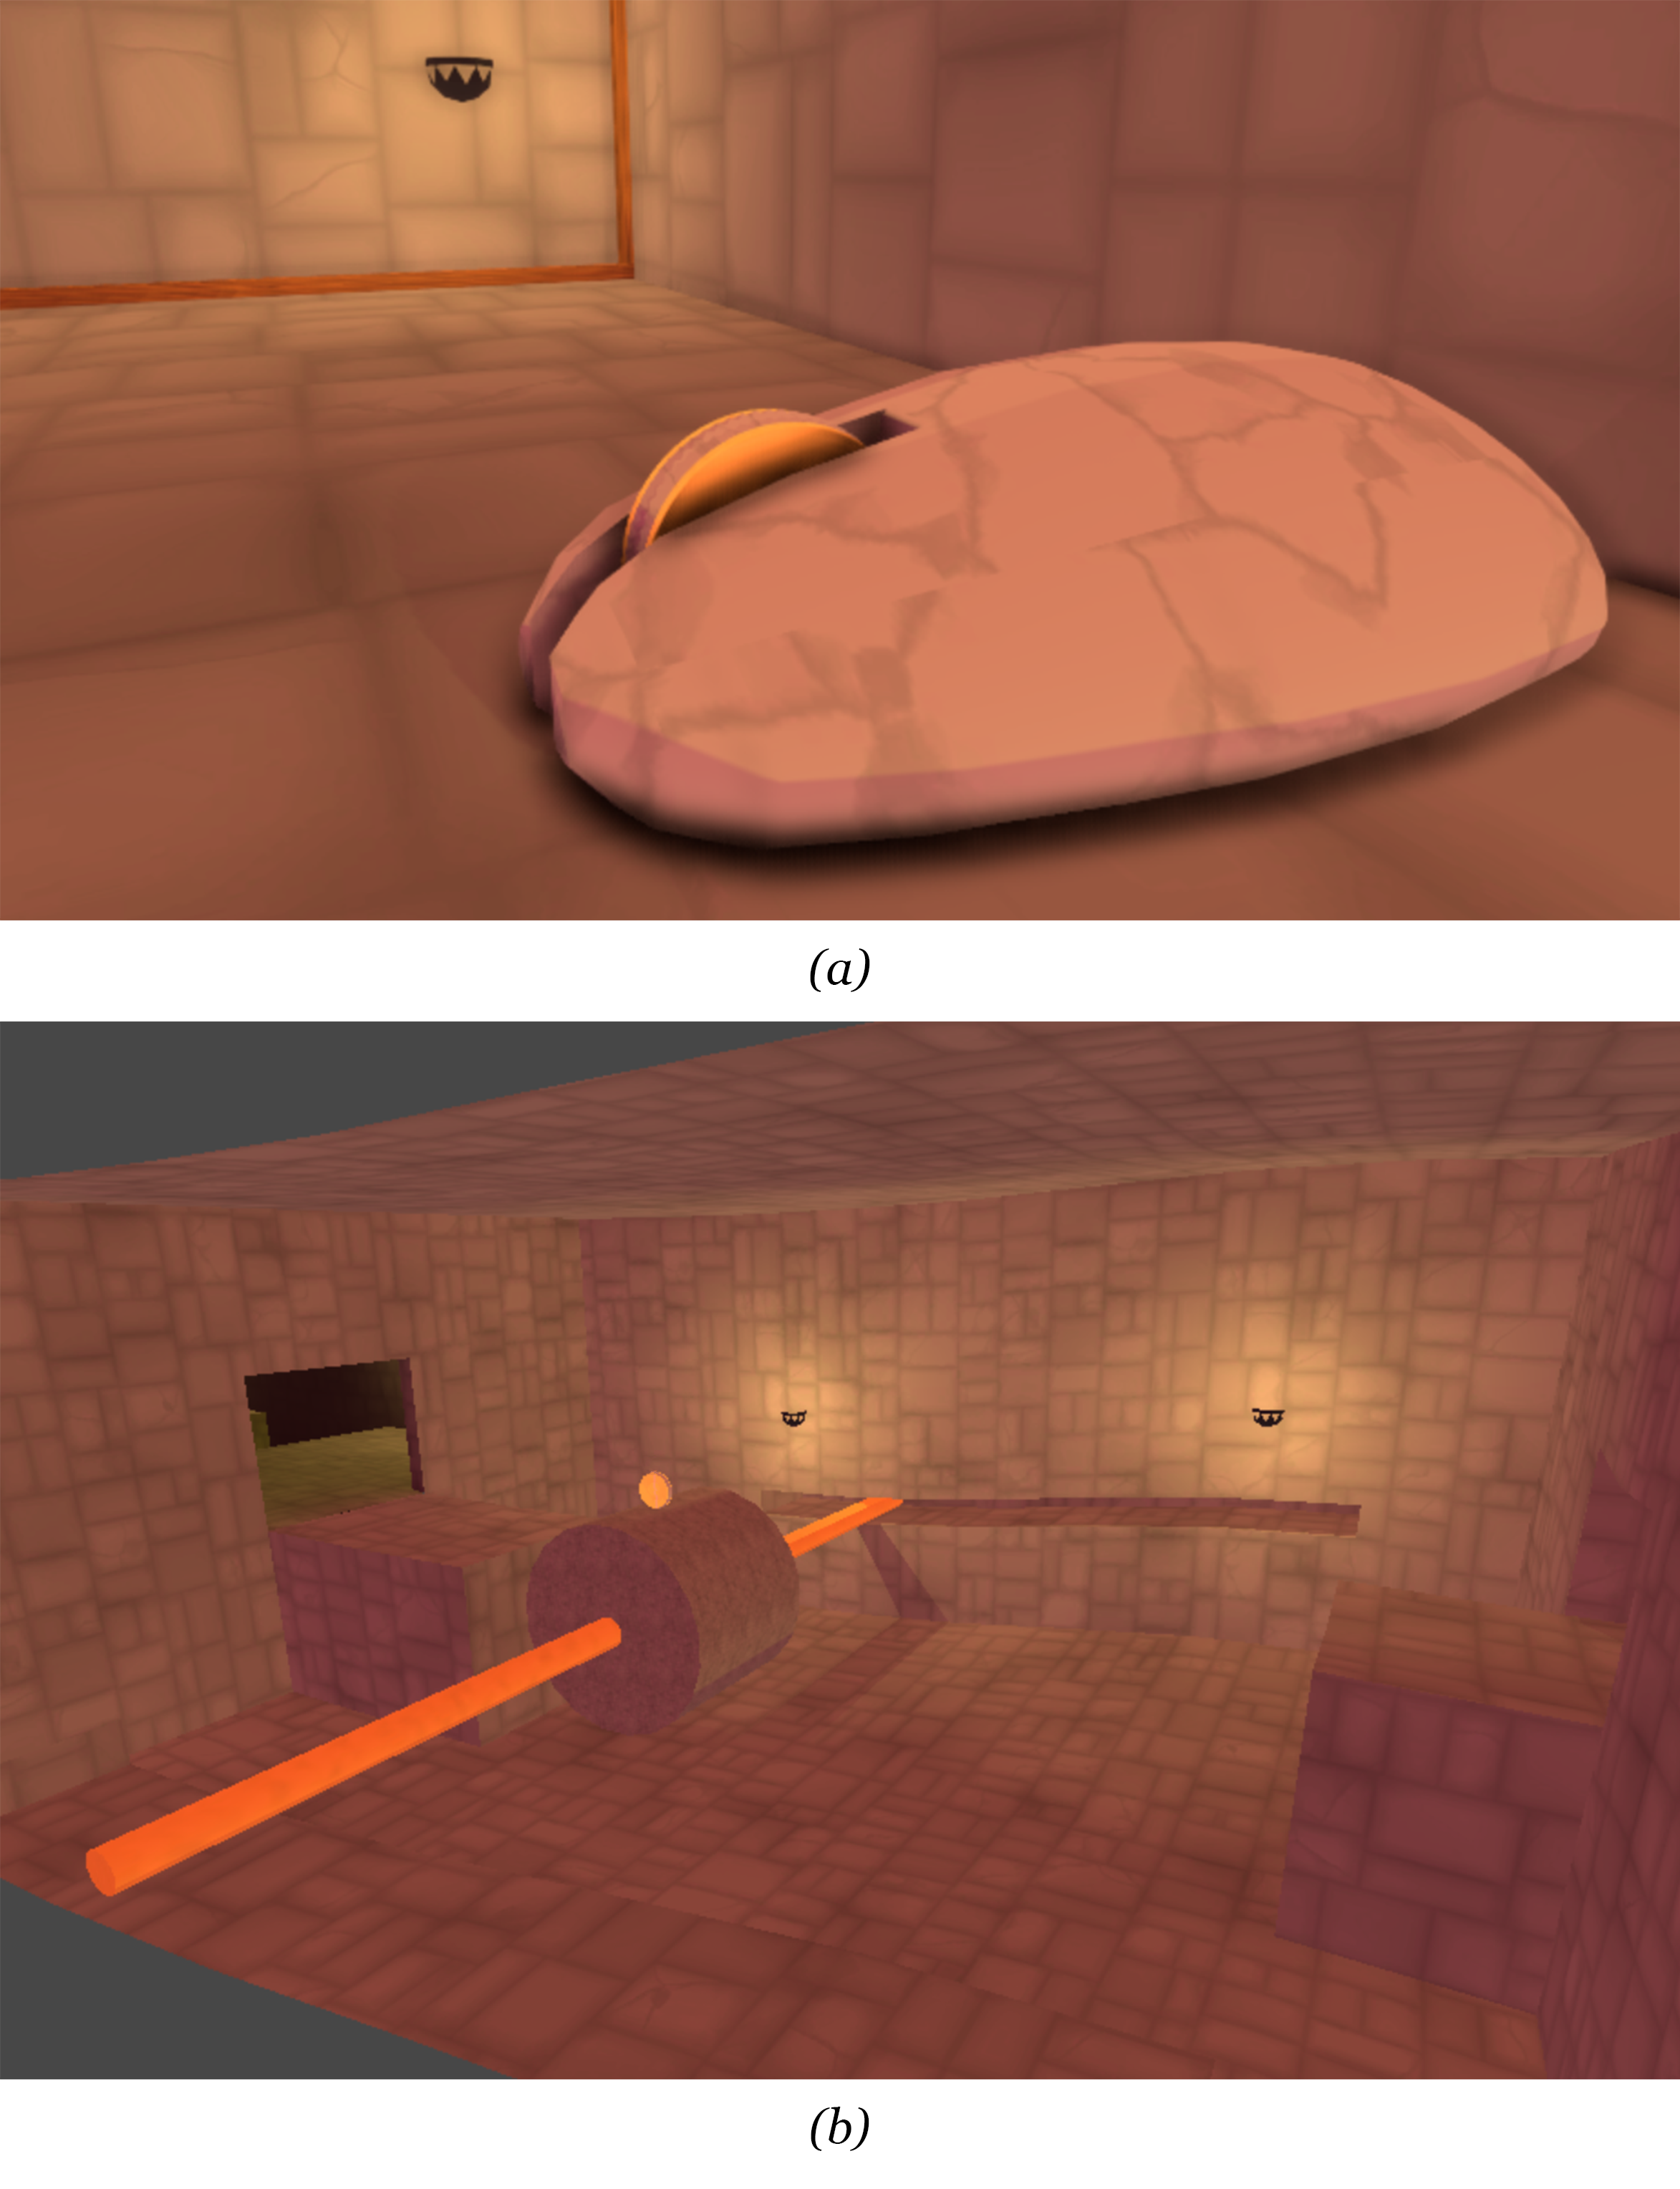
\includegraphics[width=0.6\textwidth]{PrototypeBoth}
  \caption{(a) In-game photo of the prototype as it is presented to a new player (b) The kinaesthetic challenge in focus}
  \label{prototype}
\end{wrapfigure}

Summing up, the described challenge acted as the focal point of the application phases of playtesting and ideation while the method as a whole was the focus of the last evaluation phase with the focus group interview. The next two sections will address the substance of the proposed method and the relevant findings during the two first phases of application and the impressions of the participants from the last evaluation phase. They will be divided into sections representing the context of their use: playtesting and ideation.

\subsection{A Playtest}
The workload of identifying relevant information regarding the six aspects of time, location, direction, modality, dynamics and expression from the framework has been delegated to a playtesting phase in the simplified method. The way this is done is that the interviewer conducting the playtest adhere to a number of questions during the playtest. The questions are divided into two parts: before the identified challenge is attempted and right after. These two phases reflect the phases of pre-action and post-action in the framework and are thereby related to perceivable feedforward and feedback. The questions have been formulated to echo the six aspects in a feedforward setting and a feedback setting and are preluded by a contextual question limiting the scope of the following questions totalling the questions to 14. Each question is, additionally, asked with relevance to both the physical world and the game world, so each question can be said to be two-fold, thereby covering the two dimensions of the framework.

\begin{enumerate}
  \item \textbf{Feedforward}
  \begin{enumerate}
    \item What action would you invoke to overcome the challenge?
    \item When would you apply this action and when would you stop?
    \item Where would you apply this action?
    \item In what direction would you apply this action?
    \item Is there something visually, audibly or tangibly that instructs you how to apply this mechanic?
    \item How much force, speed or acceleration do you think you need to apply?
    \item Do you think you need to apply a certain kind of attitude when applying the action?
  \end{enumerate}
  \item \textbf{Feedback}
  \begin{enumerate}
    \item Now that you have invoked the action, do you feel it was effective in overcoming the challenge?
    \item Did you feel that the action and the effect happened synchronously?
    \item Did you feel that the action and the effect happened at the same location?
    \item Did you feel that the direction of the action was parallel to the direction of the effect?
    \item Did you feel that there was any visual, tactile or audible feature that arose as a consequence of your action?
    \item Did you feel that the amount of force/speed/acceleration from your action was apparent in the effect?
    \item Did you feel that the attitude you applied in your action was apparent in the effect?
  \end{enumerate}
\end{enumerate}

As the questions were formulated they were evaluated by using them in the context they were created for: a playtest. The focus of the playtest was, as discussed earlier, the challenge in the constructed prototype. The way the playtesting was conducted was that I sat down with each participant separately and let them play through the first three minor challenges without instructing them in anything other than letting them know that at a point, I would stop them and ask them some questions. As the playtesting participant reached the challenge in focus I asked them to halt the movement of the playable figure and allowed them to look around in the game world without progressing the challenge. With the game still running, I went through the first seven questions in the given order, waiting for the participant to answer each accordingly. Each question was additionally followed up by a request for elaboration, mostly by asking why they answered what they did. As the participants answered, I wrote down their answers in the form of notes to be used as collected data in the ideation phase. As the final question was discussed I gave back the reins with the encouragement of applying the action they answered the first question with. If the action was successful in overcoming the challenge I carried on with the last seven questions, if not I asked the first seven questions once more, this time with the participant having gained new knowledge.

What was clear from the perspective of the interviewer was that the universal nature of the questions led to some of the questions seeming trivial. As an example, when inquiring about the questions regarding time (1b and 2b), as an interviewer, I was awaiting an affirmative answer, not expecting any other reply, and as a consequence, a feeling of the question as being unconstructive arose. This same consideration was also voiced during the focus group interview. Here, the participants suggested that the playtesting interview should be conducted in a semi-structured way with the questions acting as a starting point, but as the interview goes on the interviewer follows the flow of conversation. This suggestion, in addition to a suggestion of digging even deeper in elaboration on some questions like dynamics and modality (1e, 1f, 2e and 2f), I welcome. What is apparent from the test is that the questions should be considered a checklist to be answered through relevant discussion between the interviewer and the playtester in no particular order other than the first question in each section being asked first.

With that said, this alteration requires diligence of the interviewer since the task of categorising the data becomes more complex, but most importantly keeping on-topic becomes of high importance. It is possible to disregard these two tasks, but let me provide one argument for each task for why they should not: (1) The task of categorisation should not be disregarded because the categorisation inherently provides information on where a weakness or a strength in the design lies and if disregarded can lead to designers focusing on coupling on an aspect that is inappropriate for what the playtester actually experienced. Vice versa, the task of categorisation could be given to the designers, leaving them to code the data \cite{cresswell}. What is inappropriate with this approach is that tacit knowledge from the actual playtesting situation is lost \cite{cresswell}.

Conclusively, I suggest that the categorisation task should be prioritised and should be conducted by the interviewer as close in time to the playtesting as possible. (2) The task of keeping on-topic should not be disregarded because the scope of the method is relatively narrow. What can happen if the subject matter is deprioritised is that the playtesting session can evolve into a general playtesting session with discussions concerning graphical glitches, similarities to other games, aesthetic qualities, etc. which can end up being irrelevant for the purpose of the playtest, which is to gather data on the intuitiveness of a kinaesthetic challenge.

One other interesting finding was the difficulty of the participants to express and identify what they felt and why they felt the way they did. This lead to interesting replies such as when asked how much force, speed or acceleration they thought they would need to apply in the context of scrolling the mouse wheel fast enough to use the barrel as a ramp for the playable figure, the participant answered that he thought he would need as much force as one would apply to get to the bottom of a webpage. This can be explained by the fact that the method, as well as the framework, is highly concerned with knowledge residing in the lebenswelt \cite{dourish}: the intersubjective unconscious knowledge and understandings gained from experience. This knowledge is tacit knowledge in the way that it is hard to explain to another person. What makes this example so important is that intersubjectivity is used to answer the question in a way that many would understand because most have experienced the situation of wanting to scroll to the bottom of a page: It is forceful and fast. From this finding, I suggest that any utilisation of the proposed method include an explanation from the interviewer in the playtesting processes of the possibility of using past experiences as examples to identify what is felt and how it is felt.

\subsection{An Ideation}
After data has been collected, the task of plotting the data into a model to get a visual representation of what is perceived is undertaken in the ideation process of a development team or, in a bigger studio, the design team. The model for the proposed method has been considerably simplified relative to the framework. The most noteworthy simplification has been the collapse of the dimensions of feedforward and feedback. This was done as a consequence of wanting to adapt the framework into a nimble straightforward method that is accessible enough to use, that it can be a tool in a practical setting. This was done because I wanted to adapt the framework into a method for sketching \cite{buxton}. Why that had to cost the distinction between feedforward and feedback is grounded in what was earned from the distinction. In the framework, the distinction makes it clear whether or not a challenge is feedforward or feedback heavy, the analytical gain of this should be obvious and the notion that \citeA{frogger} themselves made distinctions mainly for the purpose of analysis \cite[p. 5]{vermeulen} reassures my decision, because, as a tool for sketching, the purpose of sketching is not for the sake of analysis but to spark ideas and open up a design: ``Their value lies not in the artifact of the sketch itself but in its ability to provide a catalyst to the desired and appropriate behaviors, conversations, and interactions'' \cite[p. 113]{buxton}.

Additionally, being able to look at a design challenge holistically can create better products \cite{buxton}, and this is counteracted if the designers were to make an incision at a point in the challenge and say from this point feedforward and feedback relates. With this said, there is value lost in the collapse. A value that is also relevant for a design team, and I leave it up to future interpretations to find a way to feed this value from the framework into the method. Perhaps a last analytical phase could be beneficial to a design team.

All other changes have been made to ease the drawing of a model to be used in the method, most importantly reducing the complexity of shapes. This decision should not be brushed off as just being a whimsical side note. When pen and paper sketching is such a wide-used method of sketching in a world with increasing technological gadgets promising to enhance the sketching experience, it is because grabbing a pen and a piece of paper is accessible. No app is needed, no processing power is required other than one's own brain. This is why I have put effort into reducing the framework into three lines: they are fast to draw and do not require accurate brush strokes, meaning that they can hopefully be drawn over and over in the same sketching session without becoming a nuisance. The model can be seen in figure \ref{fart}. Because of the model's resemblance to a bending river I have chosen to name the method \textit{the Four-Angled River Technique} (FART) for purposes of simple reference. From the top left in a clockwise order, the letters represent inherent information, functional information, augmented information, ludic action and action.

\begin{wrapfigure}{i}{0.5\textwidth}
  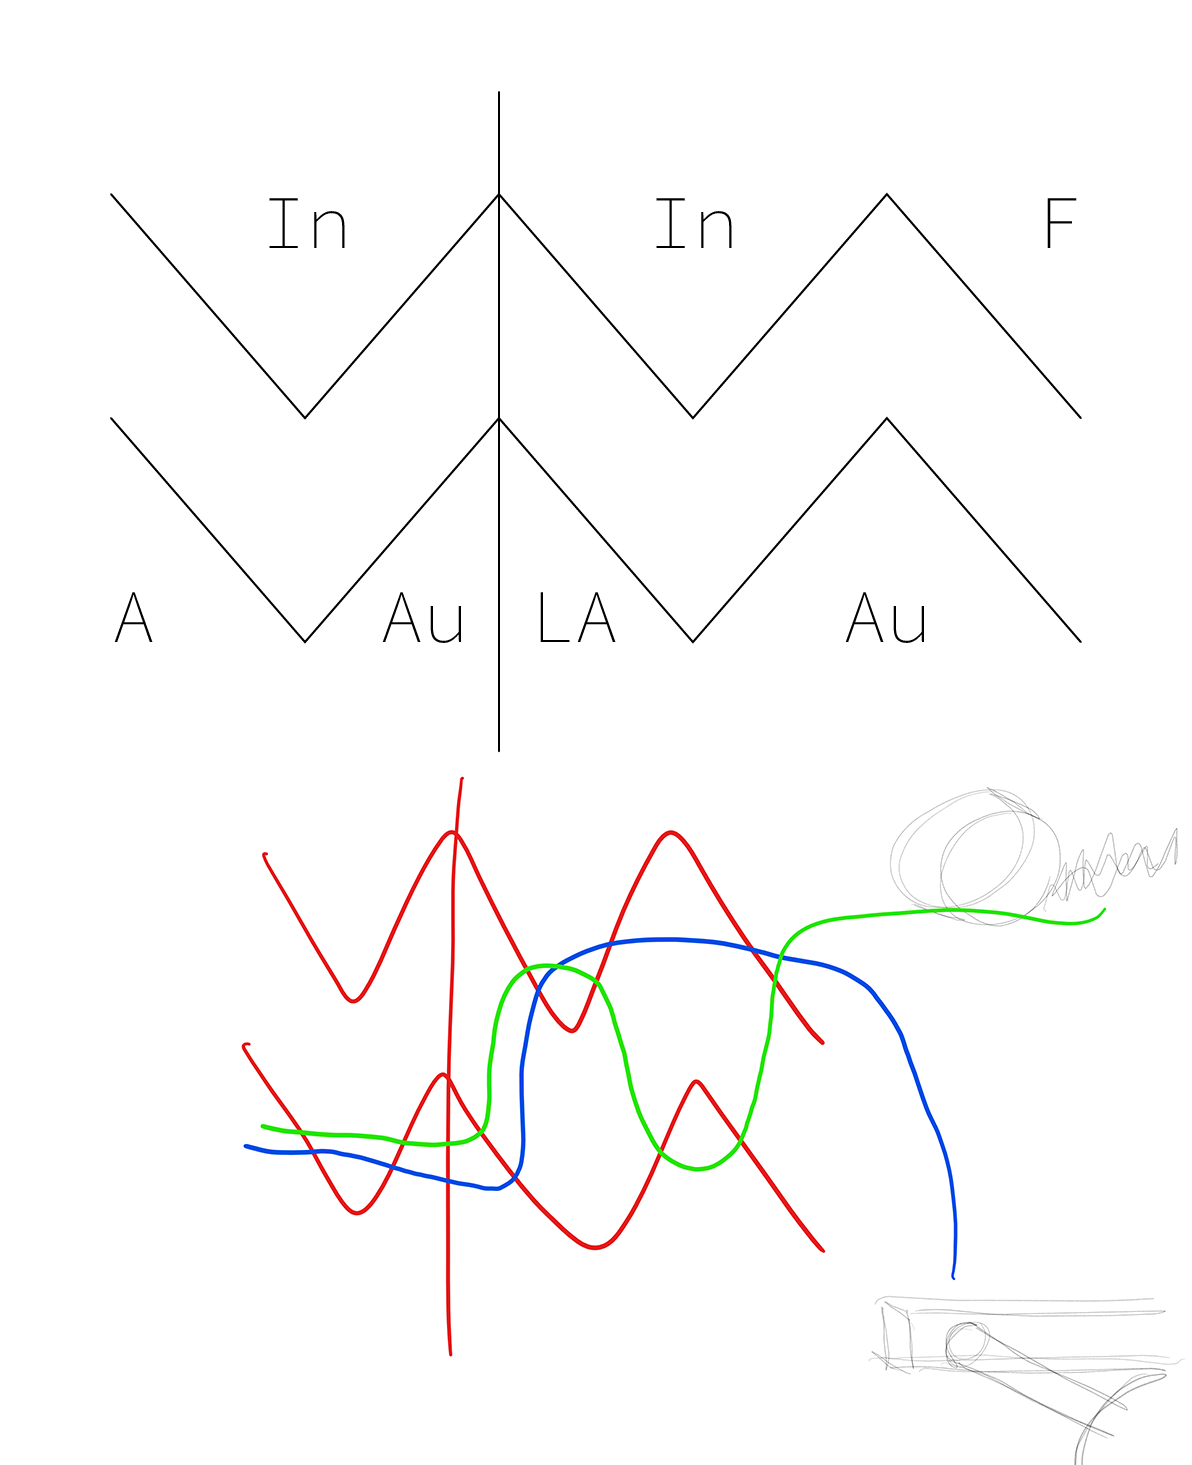
\includegraphics[width=0.5\textwidth]{FARTBoth}
  \caption{The Four-Angled River Technique. Above is the formal form and below is how it could look in practice}
  \label{fart}
\end{wrapfigure}

Before presenting the method to the participants I conducted a short lesson in the meaning of inherent, augmented and functional information. During the lesson I mirrored the notion of \citeA{frogger} in saying that inherent information is preferred over augmented information because of the lesser effort needed for psychomotor tasks compared to cognitive tasks, which means a task requires less attention, thereby allowing for internalising the controls \cite{calleja}. While promoting inherent information, a point was also made that should an inherent solution be too costly, augmented information is still preferred over no coupling, and may, in some situations, be more appropriate.

After the lesson, I presented them to the method and drew the model (see figure \ref{fart}) on an adjacent whiteboard. I then provided them with the data I had gathered from the playtests and presented them with a task: With the data and their own impressions, they should come up with ideas to improve the design of the kinaesthetic challenge from my prototype using the method. In effect, they were to role-play as a design team tasked with improving a design.

What I noted when observing the participants was that an initial confusion of how the couplings were to be visually represented was slowly replaced by a more fluid workflow of discussion and drawing. One thing that stood out, was that no lines were connected to functional information and no couplings were made between augmented and inherent information. From this I draw two conclusions: (1) The identification of functional information becomes implicit in the context of focusing on conveying meaning of how to overcome a challenge. In a sense, all ideas with the intent of making the general purpose clear to the user can be labelled as ideas providing functional information \cite{frogger}. Therefore, starting a coupling from the visual representation of functional information can seem redundant, when in fact it is not. A coupling is made between action and meaning through inherent information and augmented information. This leads me to the second conclusion: (2) The lesson was insufficient in teaching the proper skills needed to take full advantage of the method. First, the lesson should have provided the information discussed in the first conclusion and the addition that couplings are made between action or ludic action and functional information through augmented and inherent information, not between individual information types. This way of thinking of a coupling as a stream of information travelling through delineating channels may be beneficial for the understanding of the value of the method. Secondly, the lesson, as it was, focused on augmented information, inherent information and how they are distinct from each other. It should have also provided information on, not just that it can, but \textbf{how} a coupling can travel through both types of information, as was the case in the analysed example from \textit{The Legend of Zelda: Skyward Sword} where the affordance between the sword and the Deku Baba provided a coupling that travelled through augmented information and inherent information. Finally, the lesson should have provided an exemplary demonstration of how the method could be used with a dissimilar challenge to show the participants how the method is intended to be used, but with emphasis on the possibility of interpretation.

In the focus group interview that followed, granularity was a meaningful topic. One participant voiced the opinion that he would have preferred a way to label the couplings according to what the information was regarding in order to better compare different ideas. Other participants counterargued that this was against the purpose of a sketching tool, echoing the notion from \citeA{buxton}, as discussed earlier, with the sketch as an artefact having no value other than the inspirational value it provided in the creation of it. Agreeing with the majority of the participants, there still lies some truth in the one's suggestion since being able to discern the existing couplings would perhaps elevate the conversation by having recognisable couplings to relate to while sketching new ones. Again, I leave it up to future interpretations to explore the possibility of including a way of labelling information, however, using the words of \citeA{buxton}, when the pen reaches the end of a line representing a coupling, ``if you can’t afford to throw it away when done, it is probably not a sketch'' \cite[p. 111]{buxton}. Other than the point of labelling, the participants considered the method as sufficient in its granularity and expressed that the level of detail should be kept to the current minimum for the method to be constructive in an ideation process.



\section{Prototype}

Establishing criteria of rigour and relevance in interaction design research: Fallman \& Stolterman
What do prototypes prototype: Houde \& Hill
Prototypes and Prototyping in Design Research: Wensveen \& Matthews

\subsection{Use of the Framework}


\section{Tests}
Focus Group



\newpage
\bibliography{references}

\appendix
\chapter{Transcript}

Transcript from tests


\end{document}
